 \documentclass[letter,12pt]{article}
%
\usepackage[left=1in, top=1in, bottom=1in, right=1in]{geometry}

% packages 
\usepackage{latexsym,amssymb,amsmath,color}
%\usepackage{theorem}
\usepackage{graphicx}
%\usepackage[colorlinks=true]{hyperref}
%\hypersetup{urlcolor=blue, citecolor=red}
%\usepackage{algorithmic}
%\usepackage{algorithm}
\usepackage{cite}
\usepackage{verbatim}
\usepackage[table]{xcolor}

% -------------- macros
\newcommand{\p}{\partial}
\def\Cb{\overline{C}}

\newcommand{\R}{\mathbb{R}}
\newcommand{\N}{\mathbb{N}}
\newcommand{\cov}{\mathrm{cov}}
\newcommand{\iid}{\stackrel{iid}{\sim}}
\newcommand{\F}{\mathcal{F}}%
\newcommand{\be}{\begin{equation}}
\newcommand{\ee}{\end{equation}}
\newcommand{\bea}{\begin{eqnarray}}
\newcommand{\eea}{\end{eqnarray}}
%\newcommand{\p}{\partial}
\newcommand{\ttt}{\tilde}
%
\def\Wb{\overline{W}}
\def\td{\tilde \delta}
\def\tL{\tilde L}
\def\tU{\tilde U}
\def\tt{\tilde t}
\def\Vector#1{\mbox{\boldmath $#1$}}
\def\vH{{\Vector H}}
\def\vx{{\Vector x}}
\def\vy{{\Vector y}}
\def\vz{{\Vector z}}
\def\vj{{\Vector j}}
\def\vk{{\Vector k}}
\def\vt{{\Vector t}}
\def\ve{{\Vector e}}
\def\vb{{\Vector b}}
\def\vg{{\Vector g}}
\def\vn{{\Vector n}}
\def\vp{{\Vector p}}
\def\vr{{\Vector r}}
\def\vS{{\Vector S}}
\def\vV{{\Vector V}}
\def\vY{{\Vector Y}}
\def\vX{{\Vector X}}
\def\vv{{\Vector v}}
\def\vu{{\Vector u}}
\def\vQ{{\Vector Q}}
\def\vZ{{\Vector Z}}
\def\vN{{\Vector N}}
\def\vF{{\Vector F}}
\def\vC{{\Vector C}}
\def\vq{{\Vector q}}
\def\vom{{\Vector \omega}}
\def\vtau{{\Vector \tau}}
\def\F{{\rm\bf F}}
\def\sech{{\rm sech}}
\def\funnyzeta{\varsigma}
\def\tQ{\stackrel{\ldots}{Q}}
%
\def\Re{{\rm Re}}
\def\Sc{{\rm Sc}}
\def\Pe{{\rm Pe}}
\def\Pr{{\rm Pr}}
\def\Da{{\rm Da}}
\def\rf{{\rm ref}}
\def\eps{{\varepsilon}}
\def\ep{\epsilon'}
\def\O{{\rm O}}
\def\1{{\rm 1}}
\def\so{^{\rm (0)}}
\def\s1{^{\rm (1)}}
\def\d{{\rm d}}
\def\ttm{^{{\rm ttm}}}
\def\img{^{\rm im}}
\def\si{^{\rm si}}
%
\def\ol{\overline}
%
\def\tn{^{n}}
\def\tnm{^{n-1}}
\def\new#1{{\bf #1}}
%\def\new#1{{#1}}

\renewcommand{\L}{\mathcal{L}}
\newcommand{\Q}{\mathcal{Q}}
\newcommand{\U}{\mathcal{U}}
\newcommand{\G}{\mathcal{N}}
\newcommand{\V}{\mathcal{V}}
\renewcommand{\P}{\mathrm{P}}
\newcommand{\B}{\mathcal{B}}
\renewcommand{\vec}[1]{{\mathchoice
                     {\mbox{\boldmath$\displaystyle{#1}$}}
                     {\mbox{\boldmath$\textstyle{#1}$}}
                     {\mbox{\boldmath$\scriptstyle{#1}$}}
                     {\mbox{\boldmath$\scriptscriptstyle{#1}$}}}}
\newcommand{\var}[1]{{\mathrm{Var}}\left( {#1} \right)}
\newcommand{\normim}[1]{\left\| {#1} \right\|_{\scriptscriptstyle L^{2}(\Omega^{*})}}
\newcommand{\avemu}[1]{\mathrm{E}\left({#1}\right)}
\newcommand{\ave}[1]{\left\langle {#1} \right\rangle}
\newcommand{\prob}[1]{\mathrm{Prob}\left\{ {#1} \right\}}
\newcommand{\ind}[1]{\mathrm{\chi}_{\scriptscriptstyle {#1} }}
\newcommand{\NISP}{\mathcal{S}}
\newcommand{\xxi}{\vec{\xi}}
\newcommand{\ip}[2]{\left( {#1}, {#2} \right)}
\newcommand{\ipmu}[2]{\left( {#1}, {#2} \right)_\mu}
\newcommand{\norm}[1]{\left\| {#1} \right\|_{\scriptscriptstyle L^{2}(\Omega)}}
\newcommand{\normone}[1]{\left\| {#1} \right\|_{\scriptscriptstyle 1}}
\newcommand{\pard}[2]{\frac{\partial{#1}}{\partial{#2}}}
%
%\newcommand{\be}{\begin{equation}}
%\newcommand{\ee}{\end{equation}}
%\newcommand{\bea}{\begin{eqnarray}}
%\newcommand{\eea}{\end{eqnarray}}
%\newcommand{\p}{\partial}
%\newcommand{\ttt}{\tilde}
%
\def\Wb{\overline{W}}
\def\td{\tilde \delta}
\def\tL{\tilde L}
\def\tU{\tilde U}
\def\tt{\tilde t}
\def\Vector#1{\mbox{\boldmath $#1$}}
\def\vH{{\Vector H}}
\def\vx{{\Vector x}}
\def\vy{{\Vector y}}
\def\vz{{\Vector z}}
\def\vj{{\Vector j}}
\def\vk{{\Vector k}}
\def\vt{{\Vector t}}
\def\ve{{\Vector e}}
\def\vb{{\Vector b}}
\def\vg{{\Vector g}}
\def\vn{{\Vector n}}
\def\vp{{\Vector p}}
\def\vr{{\Vector r}}
\def\vS{{\Vector S}}
\def\vV{{\Vector V}}
\def\vY{{\Vector Y}}
\def\vX{{\Vector X}}
\def\vv{{\Vector v}}
\def\vu{{\Vector u}}
\def\vQ{{\Vector Q}}
\def\vZ{{\Vector Z}}
\def\vN{{\Vector N}}
\def\vF{{\Vector F}}
\def\vC{{\Vector C}}
\def\vq{{\Vector q}}
\def\vom{{\Vector \omega}}
\def\vtau{{\Vector \tau}}
\def\F{{\rm\bf F}}
\def\sech{{\rm sech}}
\def\funnyzeta{\varsigma}
\def\tQ{\stackrel{\ldots}{Q}}
%
\def\Re{{\rm Re}}
\def\Sc{{\rm Sc}}
\def\Pe{{\rm Pe}}
\def\Pr{{\rm Pr}}
\def\Da{{\rm Da}}
\def\rf{{\rm ref}}
\def\eps{{\varepsilon}}
\def\ep{\epsilon'}
\def\O{{\rm O}}
\def\1{{\rm 1}}
\def\so{^{\rm (0)}}
\def\s1{^{\rm (1)}}
\def\d{{\rm d}}
\def\ttm{^{{\rm ttm}}}
\def\img{^{\rm im}}
\def\si{^{\rm si}}
%
\def\ol{\overline}
%
\def\tn{^{n}}
\def\tnm{^{n-1}}
\def\new#1{{\bf #1}}
\newcommand{\todo}[1]{\scshape\color{red}{#1}}
%
 \def\ol{\overline}
 \def\no{\noindent}
 \def\qd{\dot{Q}}
% ----------------- end macros

\usepackage[table]{xcolor}
\usepackage{relsize}
\usepackage{bm}
\usepackage{mathrsfs}

 \def\ol{\overline}
 \def\no{\noindent}
 \def\qd{\dot{Q}}
%%%%%%%FLOW DIAGRAM%%%%%%%%%%
\usepackage[latin1]{inputenc}
\usepackage{tikz}
%\usepackage[table]{xcolor}
\usetikzlibrary{shapes,arrows}
% Define block styles
\tikzstyle{decision} = [diamond, draw, fill=blue!20, 
   text width=5.0em, text badly centered, node distance=3cm, inner sep=0pt]
\tikzstyle{block} = [rectangle, draw, fill=cyan!20, 
   text width=9.0em, text centered, rounded corners]
\tikzstyle{line} = [draw, -latex']
\tikzstyle{cloud} = [draw, ellipse,fill=red!20, node distance=3cm,
   minimum height=2em]
%%%%%%%%%%%%%%%%%%%%%%%%%%

%-------------------------------------------------------------------
\begin{document}

\thispagestyle{empty}
\begin{center}
\textsc{
Derivative-based global sensitivity approach to efficient surrogate modelling
with Polynomial Chaos
}

\bigskip 
\bigskip 

Manav Vohra$^{1}$, Alen Alexanderian$^{2}$, Cosmin Safta$^{3}$, Sankaran Mahadevan$^{1}$

\bigskip
\bigskip

\normalsize
$^1$Department of Civil and Environmental Engineering\\
Vanderbilt University\\
Nashville, TN 37235\\

\bigskip

$^2$Department of Mathematics\\
North Carolina State University\\
Raleigh, NC 27695\\

\bigskip

$^3$Sandia National Laboratories\\
Livermore, CA 94550\\

\end{center}

\vspace{6cm}

\begin{tabbing}
Corresponding Author: \hspace{5mm} \= Sankaran Mahadevan\\
       \>  Department of Civil and Environmental Engineering\\
       \>  Vanderbilt University\\
       \>  272 Jacobs Hall, VU Mailbox: PMB 351831 \\
       \>  Nashville, TN 37235 \\
       \> \\
Phone: \> (615) 322-3040 \\
Fax:   \> (615) 343-3773 \\
Email: \>  sankaran.mahadevan@vanderbilt.edu   \\
\\
Submitted to: \> \textit{Reliability Engineering and System Safety} \\
\>  May 2018\\

\bigskip
\end{tabbing}

\clearpage



\baselineskip=22pt

\tableofcontents

\section*{Abstract}
We develop a systematic approach for surrogate model
construction in reduced input parameter spaces.
%using derivative-based global sensitivity measures~(DGSMs)~\cite{Sobol:2010}. 
%
A sparse set of model evaluations in the original input space is used to  
approximate derivative based global sensitivity measures (DGSMs) 
for individual uncertain inputs of the model.
An iterative screening procedure is developed that exploits DGSM estimates in
order to identify the \emph{unimportant} inputs. The screening procedure forms
an integral part of an overall framework for adaptive construction of a
surrogate in the reduced space. The framework is tested for computational
efficiency through an initial implementation in simple test cases such as the
classic Borehole function, and a semilinear elliptic PDE with a random source
term. 
%Motivated by these experiences, the framework is fully implemented to
The framework is then deployed for a realistic application from chemical
kinetics, where we study the ignition delay time in an H$_2$/O$_2$ reaction
mechanism with 19 uncertain rate constants.  It is observed that significant
computational gains can be attained by constructing accurate low-dimensional
surrogates using the proposed framework.
 

\clearpage

\section{Introduction}
\label{sec:intro}

%\begin{enumerate}
%\item Need for efficient Surrogates - especially for complex models to enable forward UQ, 
%sensitivity studies, calibration, and experimental design (Include citations).
%\item Computational Hurdles: Polynomial Chaos and GP can be computationally 
%intractable and suffer from the curse of dimensionality (Include plots for PCE
%to motivate dimension reduction with citations for both PCE and GP).
%\item Sensitivity analyis - a potent tool for dimension reduction. However, SA can be
%computationally prohibitive. In fact, there are studies demonstrating the use of 
%surrogates to reduce costs associated with SA (include citations). 
%\item DGSM - brief introduction and citations. 
%\item Key contributions of the paper: 1) Methodology that exploits DGSM to reduce the
%dimensionality of the problem and thus enables efficient construction of surrogates.
%2) Application of the proposed methodology to investigate relative importance of
%parameters in the stillinger-weber potential, commonly used for studying phonon transport in silicon. Further, construct a reasonably accurate PC surrogate in the reduced 
%space and demonstrate computational advantage of this approach. .
%\end{enumerate}

The emerging field of uncertainty quantification (UQ) aims at methodologies for 
incorporating, characterizing, quantifying, propagating, and reducing the 
uncertainties associated with predictive models and simulations. For situations
involving complex physical models and compute-intensive simulations, an
efficient approach to construction of model surrogates is sought to enable UQ
in a tractable manner. Polynomial chaos expansion 
(PCE)~\cite{Xiu:2002,Ghanem:2003,Eldred:2008,Olivier:2010} and 
Gaussian Process (GP)~\cite{Rasmussen:2004} or Kriging~\cite{Stein:2012} are
among the most commonly used surrogates for scientific applications. However,
both approaches quickly become prohibitive when the set of uncertain model
inputs and parameters is large-dimensional. Specifically, in the case of a PCE,
a $d$-dimensional polynomial basis with a total order of truncation, $p$ 
requires model realizations at $(p+1)^d$ quadrature nodes to estimate the PC
coefficients using a fully-tensorized Gauss quadrature. This trend is 
illustrated below in Figure~\ref{fig:curse}.

\begin{figure}[htbp]
 \begin{center}
  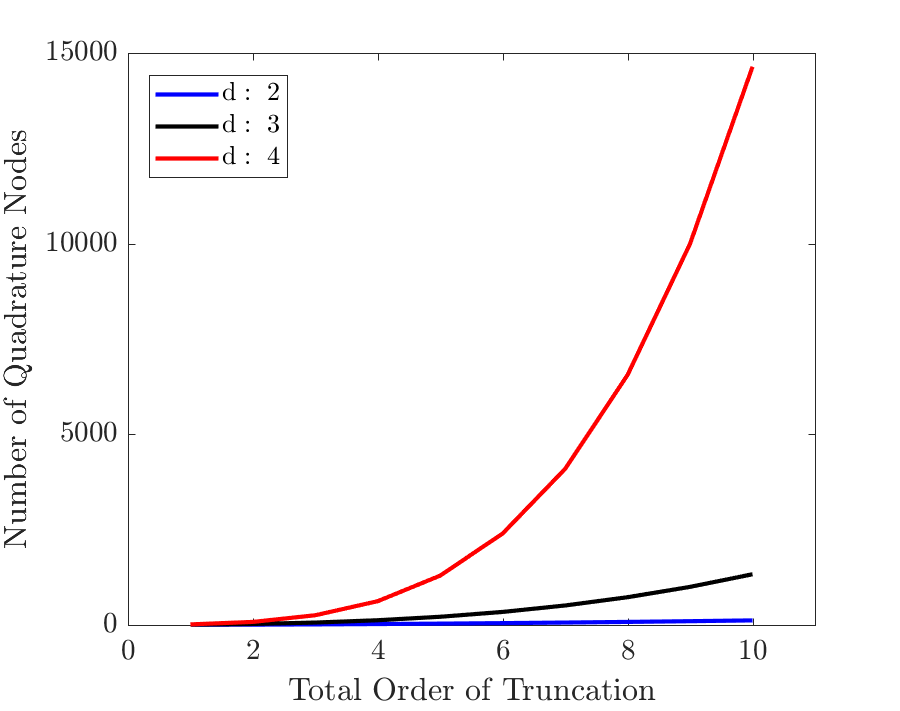
\includegraphics[width=0.70\textwidth]{./Figures/quad_comp}
\caption{Number of fully-tensorized Gauss quadrature nodes ($(p+1)^d$) is plotted against PCE total order truncation, $p$ for $d$ = 2,3, and 4.}
\label{fig:curse}
\end{center}
\end{figure}





\bigskip
\bigskip


\section{Background}
\label{sec:bg}

In this section, we introduce the notations used in the rest of
the article, and present the requisite background material on 
derivative-based global sensitivity measures and surrogate modeling 
using polynomial chaos expansion.




\subsection{Derivative-based global sensitivity analysis}  

Let $\GG$ be a mathematical model that is a function of $\Np$ uncertain 
parameters, $\theta_1, \theta_2, \ldots, \theta_\Np$. The goal of sensitivity analysis
is measuring the influence of each component of the parameter vector 
$\bm{\theta}$ on the model output. 
In the present work, we consider the case where the input parameters are statistically 
independent. 

Derivative-based global sensitivity analysis (DGSA) is performed by 
computing derivative based global sensitivity measures (DGSMs)~\cite{Sobol:2009} 
for each uncertain parameter in the model. 
Specifically, we consider the following DGSMs, 
\be
\mu_i = 
\mathbb{E}\left[\left(\frac{\partial \GG(\bm{\bm{\theta}})}{\partial \theta_i}\right)^{2}\right], \quad i = 1, \ldots, \Np.
\label{eq:mu}
\ee
Here $\mathbb{E}$ denotes expectation over the uncertain parameters.
Notice that this formulation assumes that the function $\GG$ is differentiable
with respect to $\theta_i$, $i = 1, \ldots, \Np$, almost surely.

If an analytic expression for $\GG$ is available the derivative in the above
expression can be computed directly. In applications, however, $\GG$ is often
defined in terms of a solution of a mathematical model. In some cases, 
one has access to appropriate adjoint solvers that enable efficient
adjoint-based gradient computations. In the present work, we consider
a generic computational model and only assume that the model
output depends differentiablly to the parameter $\bm{\theta}$. Thus, 
we consider finite-difference gradient computation: 
\be
\frac{\partial \GG(\bm{\theta})}{\partial \theta_i} 
\approx
\frac{\GG(\theta_1,\ldots,\theta_{i-1},
\theta_i+\Delta\theta_i,
\theta_{i+1},\ldots,\theta_d) - 
\GG(\bm{\theta})}{\Delta\theta_i}, \quad i = 1, \ldots, \Np. 
\label{eq:partial}
\ee
Then,~\eqref{eq:mu} can be evaluated by Monte Carlo sampling in
the uncertain parameter space. 
The total number of model realizations or function evaluations
needed to
compute $\mu_i$ for a function $G$ of $\Np$ random inputs and using $N$ samples is
therefore, $N\times(\Np+1)$. 
%The derivative in Eq.~\ref{eq:partial} could be evaluated
%analytically in case the functional dependence of $\GG$ and $\theta_i$
%is known. 
%Note that the perturbation $\Delta\theta_i^{*}$ is extremely small 
%compared to the uncertainty in $\theta_i$ which leads to a significant improvement
%over the `elementary effect' of a parameter, estimated in the Morris method~\cite{Morris:1991}
%using large increments.  
It is noted by many authors~[REFS], and also observed
in the numerical experiments in the present work, that a modest Monte Carlo
sample size is often sufficient for computing~\eqref{eq:mu} with reasonable
accuracy.

Consider the total 
Sobol' sensitivity index~\cite{Sobol:2001},
\be
\mathcal{T}(\theta_i) = 1 - 
\frac{\mathbb{V}[\mathbb{E}(\GG|\bm{\theta}_{\sim i})]}{\mathbb{V}(\GG)},
\label{eq:total}
\ee
where $\bm{\theta}_{\sim i}$ is the random vector $\bm\theta$ with $i$th component removed, 
and $\mathbb{V}$ denotes the variance. The total Sobol' index quantifies the total contribution 
of $\theta_i$ to variance of the model $\GG$. Components of $\bm\theta$ with small 
total Sobol' index can be considered inessential and can be fixed at nominal values. However, 
computing the total Sobol' index is a computationally expensive task for expensive-to-evaluate 
models with large number of uncertain parameters. Fortunately, 
for parameters with continuous distributions, an upper bound on $\mathcal{T}_i$  
can be expressed in terms of $\mu_i$, the Poincar\'e constant ($\mathcal{C}_i$) and the total 
variance of the model output ($\mathbb{V}(\GG)$)~\cite{Lamboni:2013}:
\be
\mathcal{T}(\theta_i) \leq \frac{\mathcal{C}_i\mu_i}{\mathbb{V}(\GG)}~(\propto \widehat{\mathcal{C}_i\mu_i})
\label{eq:bound}
\ee

\noindent The upper bound in the above inequality is proportional to the product of $\mathcal{C}_i$
and $\mu_i$. However, for the purpose of parameter screening as discussed later in
Section~\ref{sec:method}, we consider a normalized product, $\widehat{\mathcal{C}_i\mu_i}$:

\be
\widehat{\mathcal{C}_i\mu_i} = \frac{\mathcal{C}_i\mu_i}{\sum_i \mathcal{C}_i\mu_i}
\label{eq:cmu}
\ee

\noindent The Poincar\'e constant, $\mathcal{C}_i$ is specific to the probability distribution of $\theta_i$.
Table~\ref{tab:poincare} provides its value in the case of uniform and normal
distributions.
\bigskip

\begin{table}[htbp]
\renewcommand*{\arraystretch}{1.2}
\begin{center}
\begin{tabular}{|c|c|}
\hline
Distribution & $\mathcal{C}_i$ \\ \hline \hline 
Uniform, $\mathcal{U}[a, b]$ & $(b-a)^{2}/\pi^2$ \\ 
Normal, $\mathcal{N}(\mu,\sigma^2)$ & $\sigma^2$ \\ 
\hline
\end{tabular}
\end{center}

\caption{Poincare constant for the case of uniformly and normally distributed random
parameters~\cite{Roustant:2014}.}
\label{tab:poincare}
\end{table}

\subsection{Polynomial chaos expansion}

We consider models with $\Np$ random inputs, 
$\theta_1, \ldots, \theta_\Np$ that are modeled
as statistically independent random variables. The 
variables $\theta_i$ will take in physically meaningful
ranges; it is common to parameterize input uncertainties
with canonical random variables $\xi_1, \ldots, \xi_\Np$,
which can be then shifted and scaled to obtain the corresponding $\theta_i's$.
Typical choices for distribution of $\xi_i$ include standard normal 
and uniform distribution on the interval $[-1, 1]$.
Let 
\[
   \bm{f}(\bm{x}) = \prod_{i=1}^\Np f_i(x_i), \quad \bm{x} \in \mathbb{R}^\Np
\]
where $f_i$ are probability density functions of $\xi_i$, $i = 1, \ldots, \Np$.
We consider a square integrable random variable $\GG:\R^\Np \to \R$; 
that is,
\[
\int_{\mathcal{D}} \GG(\bm{\xi})^2 \, \bm{f}(\bm{\xi})d\bm{\xi} < \infty,
\]
where $\mathcal{D}$ is the support of the distribution law of the random vector
$\bm{\xi}$. 


% for representing the
%dependence of a random observable ($\GG$) on independent uncertain or
%stochastic model parameters ($\bm{\theta}$).  Considering a joint probability
%distribution of the components of ($\bm{\theta}$) as
%$\mathbb{P}(\bm{\theta})$, the following condition is imposed on
%$\GG$:
%\be
%\mathbb{E}[\GG^2] = \int_{\mathcal{D}_{\bm{\theta}}} \GG^2 \mathbb{P}(\bm{\theta}) 
%d\bm{\theta} < \infty
%\ee

%\noindent where $\mathcal{D}_{\bm{\theta}}$ is the domain of the input parameter space. 

As mentioned in Section~\ref{sec:intro}, the 
polynomial chaos expansion
(PCE) is a commonly used tool for surrogate modeling. 
The PCE of
$\GG$ is a mean-square 
convergent series expansion~\cite{Xiu:2002,Ghanem:2003,Olivier:2010} of the form:
\be
\GG(\bm\xi) = \sum_{k=0}^\infty c_k\Psi_k(\bm{\xi}),
\ee
where $\Psi_k$'s form a multivariate orthogonal polynomial
basis---orthogonal with respect to the joint probability distribution of $\bm{\xi}$.
%
In practice, a truncated expansion is used.  Moreover, in applications, $\GG$
is a mathematical model of interest that takes a parameter vector $\bm{\theta}$
(with components in physically meaningful ranges) as input. Therefore, we 
write the truncated PC representation of a model $\GG$ as follows:
\be 
\GG(\bm\theta) \approx \GG^{\mbox{\tiny PC}}(\bm\theta) := \sum_{k=0}^{\Npc}
c_k\Psi_k (\bm\xi(\bm\theta)), 
\ee
where $\bm\xi(\bm\theta)$ is found by a simple linear transformation.

Computational strategies available for estimating the PC coefficients
($c_k$'s) typically involve techniques based on projection or regression.
Projection-based methods consider the orthogonal projection of 
$\GG$ on the PC basis $\{\Psi_k\}_{k=0}^\Npc$ and compute
the resulting expansion coefficients via quadrature~\cite{Olivier:2010}.
%on numerical quadrature for estimating the
%following expectation:
%\be
%\bm{c} = \mathbb{E}[\Psi_\alpha(\bm{\xi})\cdot\GG^{\mbox{\tiny{M}}}]
%\approx
%\sum_{i=1}^{N} \GG^{\mbox{\tiny{M}}}(\bm{\theta}^{(i)})w^{(i)}\Psi_\alpha(\bm{\xi}^{(i)})
%\ee
%\noindent where $w^{(i)}$ denotes the weight associated with the quadrature node $i$. 
Regression-based methods such as least angle regression (LAR)~\cite{Efron:2004}, and least absolute shrinkage
and selection operator (LASSO)~\cite{Tibshirani:1996} aim to construct a sparse PCE~\cite{Blatman:2008}
by solving a regularized optimization problem. Specifically in the case of LAR, a penalty term comprising the L-1
norm of the PC coefficients is used:

\be
\hat{\bm{c}} = \mbox{argmin}~\mathbb{E}_{\bm\theta}
\left[\left(\sum_{k=0}^\Npc c_k \Psi_k(\bm\xi(\bm\theta)) -
\GG(\bm{\theta})\right)^{2}\right]  + \lambda\normone{\bm{c}}
\label{eq:reg}
\ee
where $\normone{\bm{c}}$ = $\sum_{k=0}^\Npc |c_k |$.
The regularization term forces the minimization towards sparse coefficient vectors resulting
in sparse PC representations.
In this work, we construct sparse PCEs with LAR using UQLab~\cite{Marelli:2014},
a general purpose uncertainty quantification software developed at ETH Zurich.
% in Switzerland.



















\bigskip
\bigskip


\section{Methodology}
\label{sec:method}

%Stage1: QoI selection for accurate estimation of derivatives and PCE, Stage 2: Parameter Screening, Stage 3: Reduced-order Surrogate Verification
%
%1. Goal is to estimate the upper bound on Sobol total-effect index using DGSM. 
%2. QoI should be differentiable w.r.t all the parameters. 
%3. Derivative could be estimated analytically or numerically.
%4. The expected value of the partial derivative w.r.t a given parameter is approximated over a few samples.
%5. Gradually enhance the sample size until some degree of convergence is established.
%6. Note that model runs at the full parameter space will be used for verification of the ROS. However, one could consider
%relaxing the convergence criterion to reduce computational costs. 
%7. Consider the product of Ci and mu_i to screen parameters.i

In this section, we outline the underlying methodology for constructing a 
reduced-order surrogate using sensitivity analysis. The term `reduced-order'
in the present context implies that the surrogate is constructed in a 
subspace that sufficiently captures the uncertainty in the model output. 
For instance, in the case of PC surrogates, the dimensionality of the polynomial
basis functions is effectively reduced. A possible approach to 
constructing a reduced-order surrogate involves sensitivity analysis of the
uncertain model parameters with respect to a given output, and thereby
disregarding the uncertainty associated with parameters considered as unimportant.
For this purpose, a global sensitivity analysis based on Sobol indices could be pursued.
However, as discussed earlier in sections~\ref{sec:intro} and~\ref{sec:bg}, determining converged 
estimates of Sobol sensitivity indices typically requires tens of thousands
of model evaluations. Consequently, the exercise becomes prohibitive in
situations where the model runs are compute-intensive. Instead, we estimate a normalized
upper-bound ($\widehat{\mathcal{C}_i\mu_i}$, see Eq.~\ref{eq:bound}) on the Sobol total
effect index ($\mathcal{T}(\theta_i)$) for each parameter, $\theta_i$, and use it as a 
metric to identify the unimportant parameters. Below, we provide an algorithm for 
parameter screening. It is assumed that the partial derivatives in Eq.~\ref{eq:mu}
are estimated using finite difference. 

\bigskip

\begin{breakablealgorithm}
  \caption{Parameter screening with derivative-based sensitivity measures.}
  \begin{algorithmic}[1]
    \Procedure{Screening}{}
      \State Generate $n_1$ points in $\mathbb{R}^{d}$.\Comment{$d$: 
             Number of uncertain model parameters.}
      \State Perturb each point along the $d$ directions to obtain a set of $n_1(d+1)$ points.
      \State Compute $\mu_i$ using model evaluations at the $n_1(d+1)$ points in Eq.~\ref{eq:mu}
      \State Determine initial ranks, $\mathcal{R}^{old}$ based on $\widehat{\mathcal{C}_i\mu_i}$ values for $\theta_i$.
      \State set $k$ = 1\Comment{Iteration counter}
      \Do
        \State Generate $n_k$ new points in $\mathbb{R}^{d}$.
        \State Perturb each point along the $d$ directions to obtain a set of $n_k(d+1)$ points.
        \State Compute and store model evaluations at the $n_k(d+1)$ points.
        \State Compute $\mu_i$ using prior model evaluations at $(d+1)(n_1 + \sum_j^k n_j)$ points.
        \State Determine new ranks, $\mathcal{R}^{new}$ based on updated $\widehat{\mathcal{C}_i\mu_i}$ values.
        \State Compute $max\_pdev$ = max$\left(\frac{|\mu_{i,k} - 
               \mu_{i,k-1}|}{ \mu_{i,k-1}}\right)$.\Comment{$max\_pdev$:
               Maximum percentage deviation in $\mu_i$ between successive iterations.}
        \State set $k$ = $k$ + 1
      \doWhile{($\mathcal{R}^{\tiny{new}}$ $\neq$ $\mathcal{R}^{\tiny{old}}$ {\bf or}  
               $max\_pdev$~$>~\tau$)\Comment{$\tau$:~Tolerance}}
    \EndProcedure
  \end{algorithmic}
\end{breakablealgorithm}

\bigskip

Based on the steps outlined in the above algorithm, it can be said that the set of sample points used for
estimating the screening metric, $\widehat{\mathcal{C}_i\mu_i}$ is enriched until consistency in ranks
between successive iterations as well as a certain degree of convergence in estimates of the screening 
metric for each uncertain parameter is accomplished. Parameter
screening is an integral part of the overall strategy for constructing the reduced-order surrogate as 
depicted below using a flow-diagram. 

\bigskip



\begin{figure}[htbp]
\begin{center}
\begin{tikzpicture}[node distance=1.5cm]

\node (start) [startstop] {Start};

\node (qoi) [io, below of=start,align=left] {Select an appropriate model output};

\draw [line] (start) -- (qoi);

\node (tol) [process, below of=qoi, text width=8em] {Set an initial tolerance, $\tau$};

\draw [line] (qoi) -- (tol);

\node (screen) [process, below of=tol, text width=9.5em] {Parameter Screening};

\draw [line] (tol) -- (screen);

\node (dr) [draw, diamond, aspect=1.5,yshift=-6.7cm, text width=4.5em, text centered] {Is DR possible$?$};

\draw [line] (screen) -- (dr);

%\node (dr_mean) [right of=dr, xshift=5cm] {DR: Dimension Reduction};


\end{tikzpicture}
\end{center}

\caption{Flow-diagram outlining the overall strategy for constructing reduced-order surrogates using
the derivative-based sensitivity measures. Note that DR is an abbreviation for dimension reduction.}
\end{figure}







 

\bigskip
\bigskip


\section{Motivating Examples}
\label{sec:examples}

In section~\ref{sec:method}, we presented a framework for constructing
an ROS (if deemed advantageous) by identifying unimportant parameters based on 
estimates of the screening metric, $\widehat{\mathcal{C}_i\mu_i}$
for individual parameters.
In this section, we motivate the underlying methodology by applying it to three
test problems,
namely, the borehole function, a non-linear oscillator, and a semi-linear elliptic PDE.
Since model evaluations in all these test
problems are inexpensive, we compare relative importance of model parameters based
on the screening metric, obtained using model evaluations with 
converged estimates of $\mathcal{T}(\theta_i)$ based on the surrogate constructed in the
full parameter space (FSS). Additionally, to illustrate computational gains, we compare
convergence trends as a function of training runs for the ROS and the FSS using 
$\epsilon_{\mbox{\tiny LOO}}$ in Eq.~\ref{eq:loo}. 
Furthermore, as discussed earlier in section~\ref{sec:method}, we compare
PDFs of the model output, obtained using the ROS and the full-space surrogate for
the purpose of verification. 

\subsection{Borehole function}

The borehole function is a benchmark reference problem in sensitivity analysis.
It models the discharge of water ($\mathcal{Q}$) through a borehole in terms of
geometrical and physical parameters:
\be
\mathcal{Q} = \frac{\displaystyle
2\pi T_u(H_u - H_l)}{\displaystyle
\ln({r}/{r_w})\Big[1 +
\frac{2LT_u}{
\ln({r}/{r_w})r_w^2K_w} + \frac{T_u}{T_l}\Big]}
\label{eq:bore}
\ee
The radius of influence, $r$ is fixed at 3698.30 m whereas all other parameters
in the right hand side of~\eqref{eq:bore} are considered 
as uncertain. Hence, $\mathcal{Q} = \mathcal{Q}(\vec{\theta})$ with 
 $\vec{\theta} = (r_w, L, T_u, H_u, T_l, H_l, K_w)^T$, a vector of
 uncertain parameters. Table~\ref{tab:bore} provides distributions of the
 uncertain input parameters. 

\begin{table}[htbp]
\renewcommand*{\arraystretch}{1.2}
\begin{center}
\begin{tabular}{ll}
\toprule
\textbf{Parameter} & \textbf{Distribution} \\ 
\bottomrule
Borehole radius, $r_w$ (m) & $\mathcal{N}$(0.1,0.016) \\
Borehole length, $L$ (m) & $\mathcal{U}$[1120,1680] \\
Transmissivity of upper aquifer, $T_u$ (m$^2$/yr) & $\mathcal{U}$[63070,115600] \\
Potentiometric head of upper aquifer, $H_u$ (m) & $\mathcal{U}$[990,1110] \\
Transmissivity of lower aquifer, $T_l$ (m$^2$/yr) & $\mathcal{U}$[63.1,116] \\
Potentiometric head of lower aquifer, $H_l$ (m) & $\mathcal{U}$[700,820] \\
Borehole hydraulic conductivity, $K_w$ (m/yr) & $\mathcal{U}$[9855,12045] \\
\bottomrule
\end{tabular}
\end{center}

\caption{Description and distributions of uncertain parameters in the borehole function
given by~\eqref{eq:bore}.}
\label{tab:bore}
\end{table}
%
Cheap function evaluations of the discharge $\mathcal{Q}(\vec{\theta})$ using
enables computing accurate estimates of $\mathcal{T}(\theta_i)$ through
sampling, with a sufficiently large Monte Carlo sample size.  Shown in
Figure~\ref{fig:sense_bore}~(left) are estimates of these indices corresponding to the
uncertain parameters in the borehole function using 10$^6$ pseudo-random
samples in the input parameter space. 
%\footnote{Although $\mathcal{T}(\theta_i)$ might converge with much fewer
%samples depending upon the model, we consider a large number that typically
%ensures a converged estimate for the purpose of illustration.} 
These estimates are used to verify fidelity of
parameter screening based on the methodology presented in Section~\ref{sec:method}. 

\begin{figure}[htbp]
 \begin{center}
  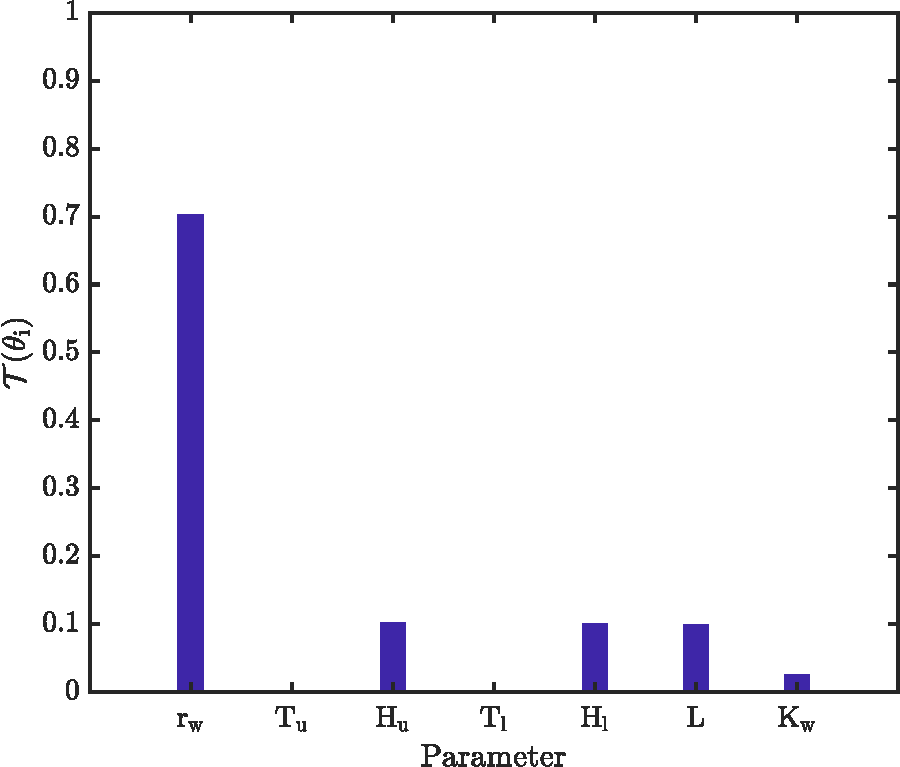
\includegraphics[width=0.48\textwidth]{./Figures/sense_borehole}
  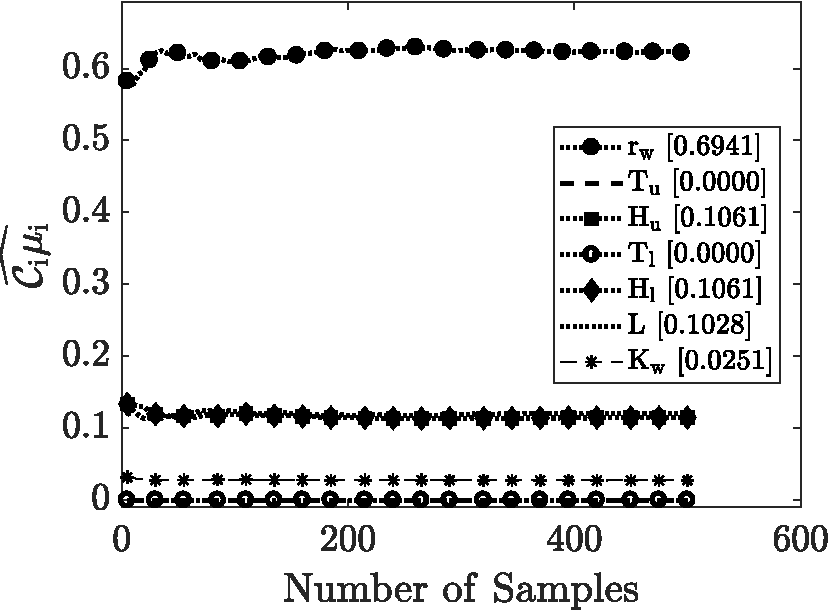
\includegraphics[width=0.51\textwidth]{./Figures/ub_conv_borehole}
\caption{
Left: Sobol' total sensitivity index, $\mathcal{T}(\theta_i)$ for uncertain
parameters in the
borehole discharge function in~\eqref{eq:bore}. Right: 
Estimates of the screening metric ($\widehat{\mathcal{C}_i\mu_i}$), plotted
against number of samples. Also included in the legend are estimates of
$\mathcal{T}(\theta_i)$ in each case in the legend.}
\label{fig:sense_bore}
\end{center}
\end{figure}

In Figure~\ref{fig:sense_bore}~(right), we plot estimates of the screening parameter 
$\widehat{\mathcal{C}_i\mu_i}$ for a wide range of the number of 
samples used for approximating $\mu_i$ using~\eqref{eq:mu}.
Estimates for $\widehat{\mathcal{C}_i\mu_i}$ are found to be in excellent agreement
with $\mathcal{T}(\theta_i)$ even when small number of samples (5--10) are used. 
Consequently, the relative importance of uncertain 
parameters in the borehole function is found to be consistent 
with predictions based on the Sobol' index. 
In the considered intervals for the uncertain parameters, it is clear 
that the discharge is insensitive to $T_u$ and $T_l$. 
Moreover, the sensitivity to $K_w$ is also small. We exploit these findings to reduce
the dimensionality of the problem by 
discounting the uncertainties in $T_u$, $T_l$, and $K_w$ by fixing 
them at their respective nominal values. 

Our goal as discussed is to gain computational advantage by constructing
surrogates in a reduced input parameter space. To this end, we use LAR to 
construct PCEs
in 5D and 4D spaces by fixing $\{T_u,T_l\}$ in the former and additionally
fixing $K_w$ in the latter at their respective mean values. In
Figure~\ref{fig:conv_bore}~(left), we compare convergence of PCEs constructed in the
full space (7D) with those constructed in the two reduced spaces (4D and 5D)
using $\epsilon_{\mbox{\tiny{LOO}}}$ (Eq.~\ref{eq:loo}). 

\begin{figure}[htbp]
 \begin{center}
  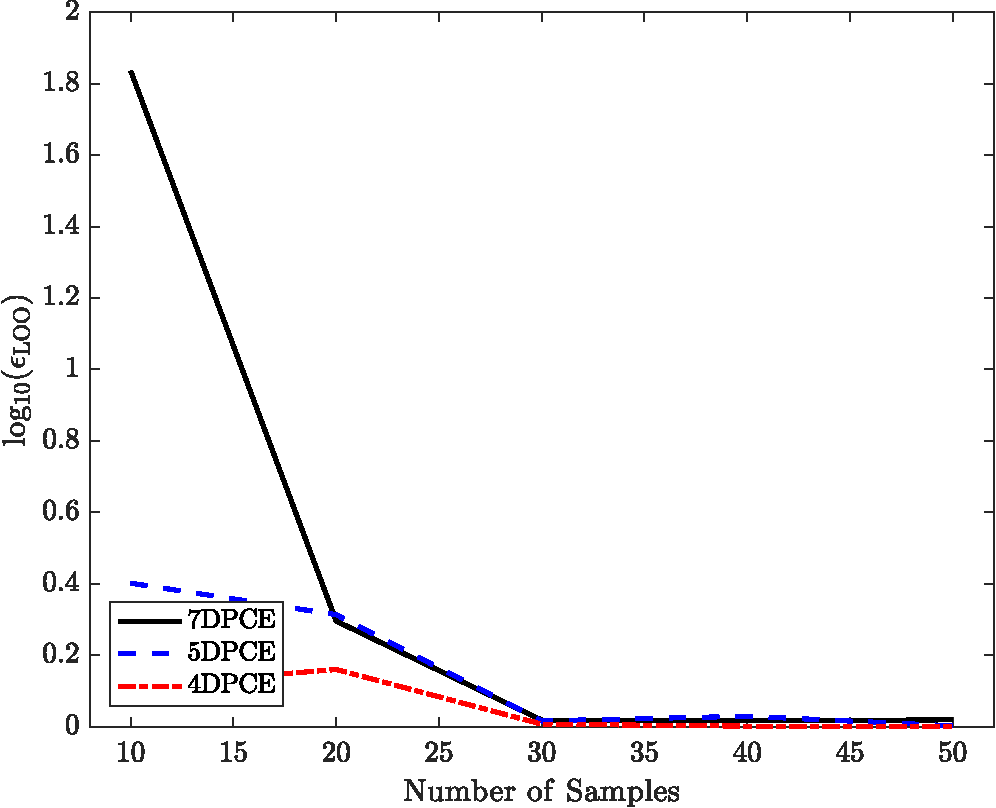
\includegraphics[width=0.48\textwidth]{./Figures/err_samples_borehole}
  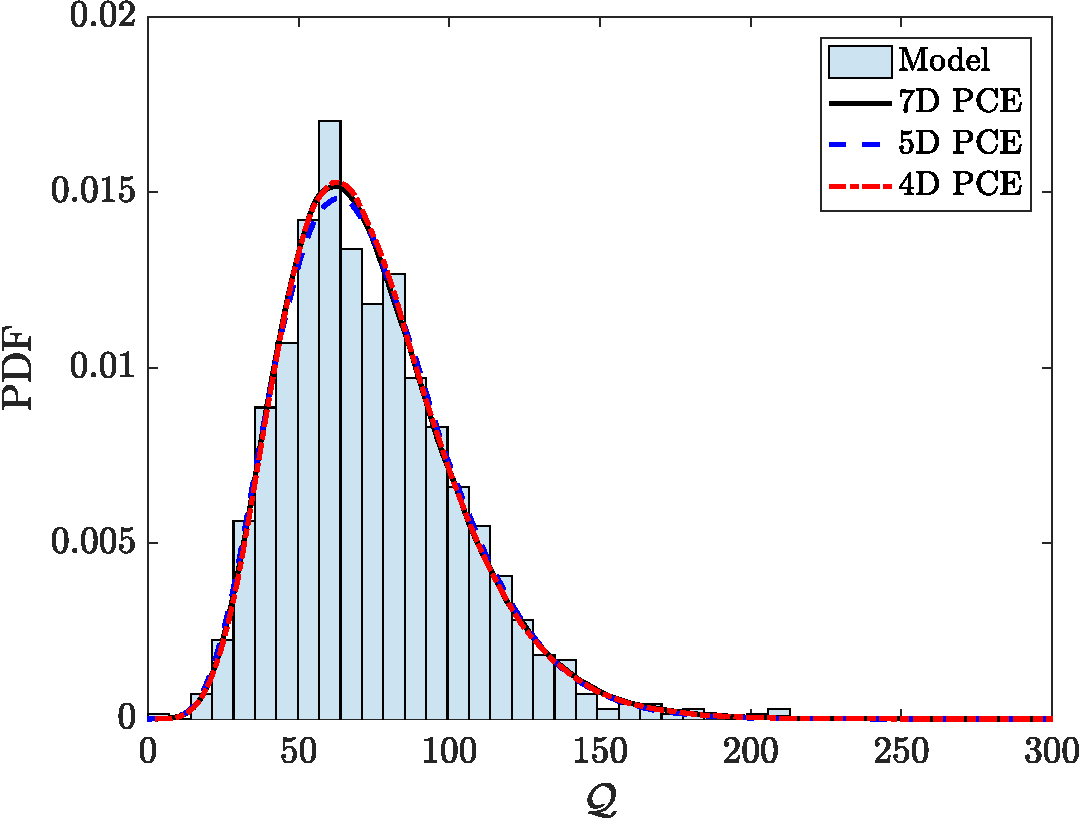
\includegraphics[width=0.48\textwidth]{./Figures/pdf_comp_borehole}
\caption{Left: A comparison of order of the leave-one-out-error 
($\epsilon_{\mbox{\tiny{LOO}}}$) as a function of number of regression samples
used for constructing the PCE in 4, 5, and 7 dimensions. Right: A comparison of
PDFs of the discharge, $\mathcal{Q}$, generated using 10$^{6}$ samples from
the marginal distributions of the uncertain parameters in each case.} 
\label{fig:conv_bore}
\end{center}
\end{figure}
%
As expected, it is observed that the PCE constructed in the 4D space converges
at a much faster rate. For instance, if a PCE with $\mathcal{O}(10^{-4})$
accuracy is sought, we need function evaluations at only about 50 sample points
in the 4D parameter space whereas the number of samples needed in the full 7D
space seems much higher. Latin hypercube sampling (LHS) was used in
each case. It must be pointed out that the error in Figure~\ref{fig:conv_bore}~(left)
is not expected to decrease monotonically with the increase in sample size
owing to the penalty term in the regularized optimization problem in Eq.~\ref{eq:reg}. 


As discussed earlier in this section, the reduced order PCE's are verified for
predictive accuracy in a least-squares sense and a probabilistic sense.
Estimates for $\epsilon_{\mbox{\tiny{L-2}}}$ based on 50 samples in the
validation test suite were
found to be 0.0551 and 0.0112 for the 4D and 5D PCE's respectively. In other
words, the 4D PCE is accurate within 5.52$\%$ and the 5D PCE is accurate within
1.12$\%$ of predictions based on the borehole function. We note  that although
the convergence in the case of a 5D PCE is slower (Figure~\ref{fig:conv_bore}),
its predictive accuracy is higher than the 4D PCE. This illustrates the
trade-off between accuracy and computational efficiency for the present 
problem. Generally, the required level of accuracy is problem dependent. 
The present framework allows for moving towards higher fidelity 
reduced order surrogates based on the ranking of the parameter sensitivities. 
 
%A possible explanation for this observation is that above a certain order
%of convergence, the uncertainty in $k_w$ contributes much more towards
%predictive accuracy of the reduced order PCE. It is therefore critical to
%account for the order of PCE convergence as well as its predictive accuracy for
%a given application, as highlighted earlier in section~\ref{sec:method}. 


Figure~\ref{fig:conv_bore}~(right) illustrates a comparison of the PDFs
of the
discharge, $\mathcal{Q}$ obtained by propagating 10$^6$ random
samples through the 7D PCE in the original input parameter domain as well as
the reduced order PCEs constructed in 4 and 5 dimensions. A normalized histogram
plot using 1000 model evaluations in the validation test suite is also included.
It is evident from this plot, that the PDFs agree quite favorably with each
other as well as the model-based histogram with respect to the modal estimate
as well as the uncertainty associated with $\mathcal{Q}$. 
Consequently, it can be said that the reduced order PCE is verified in a
probabilistic sense. In other words, the mode as well as the uncertainty in the
observable is reliably captured and predicted by the reduced order PCE. 
% 
\subsection{Nonlinear Oscillator}
We consider an undamped nonlinear oscillator with only one degree of
freedom as illustrated in Figure~\ref{fig:osc}. 
\begin{figure}[htbp]
 \begin{center}
  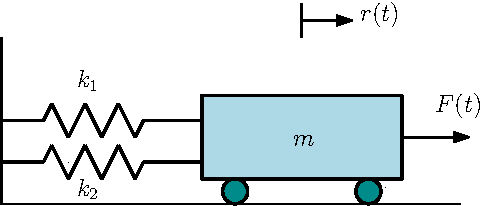
\includegraphics[width=0.5\textwidth]{./Figures/oscillator}
\caption{Schematic illustration of an undamped non-linear oscillator system with one degree of freedom.}
\label{fig:osc}
\end{center}
\end{figure}
This system has been studied extensively for its reliability using
the following state function~\cite{Bucher:1989,Bucher:1990,Rajashekhar:1993,Schueremans:2005,Gayton:2003}:
%
\be
g(\bm{X}) = 3r - \left|z_\text{max}\right| = 3r - 
\left|\frac{2F}{m\omega_0^2}\sin\left(\frac{\omega_0t_1}{2}\right)\right|,
\label{eq:limit}
\ee
\noindent where $z_\text{max}$ is the maximum displacement response of the system, $r$ denotes the displacement at
which either spring yields, $\bm{X}=(m,k_1,k_2,r,F,t_1)^T$ is the vector 
of uncertain parameters, and   
$\omega_0~=~\sqrt{(k_1+k_2)/m}$. The uncertain parameters are considered to be normally distributed with mean
and variance as provided below in Table~\ref{tab:osc}.

\begin{table}[htbp]
\renewcommand*{\arraystretch}{1.2}
\begin{center}
\begin{tabular}{ll}
\toprule
\textbf{Parameter} & \textbf{Distribution} \\ 
\bottomrule
Mass, $m$ (kg) & $\mathcal{N}$(1,0.05) \\
Time, $t_1$ (s) & $\mathcal{N}$(1,0.2) \\
Force, $F$ (N) & $\mathcal{N}$(1,0.2) \\
Displacement, $r$ (m) & $\mathcal{N}$(0.5,0.05) \\
Spring Constant, $k_1$ (Nm$^{-1}$) & $\mathcal{N}$(1,0.1) \\
Spring Constant, $k_2$ (Nm$^{-1}$) & $\mathcal{N}$(0.1,0.01) \\
\bottomrule
\end{tabular}
\end{center}

\caption{Description and distributions of uncertain parameters in the limit state function~\eqref{eq:limit}.}
\label{tab:osc}
\end{table}

Converged estimates of $\mathcal{T}(\theta_i)$ are once again obtained easily by
evaluating $g(\bm{X})$ for a large set of samples in the uncertain 
parameter space; see Figure~\ref{fig:sense_osc}~(left). Estimates of the screening metric, 
$\widehat{\mathcal{C}_i\mu_i}$ are plotted against the number of samples in 
Figure~\ref{fig:sense_osc}~(right). 
\begin{figure}[htbp]
 \begin{center}
  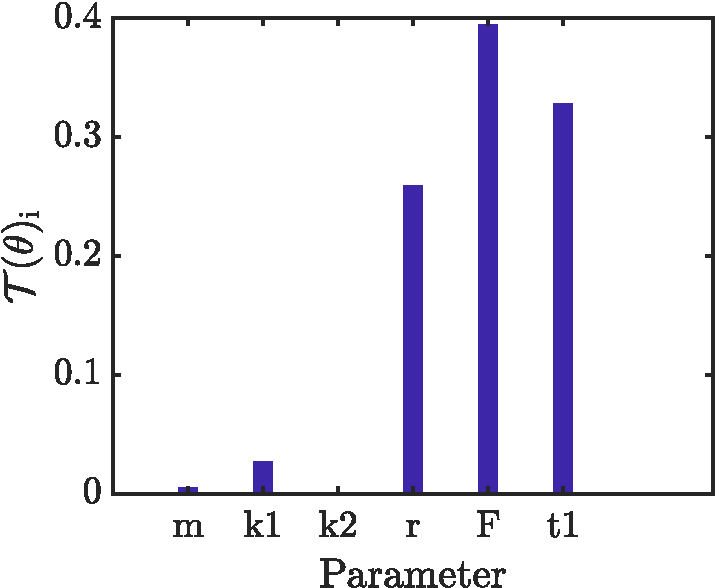
\includegraphics[width=0.48\textwidth]{./Figures/sense_oscillator}
  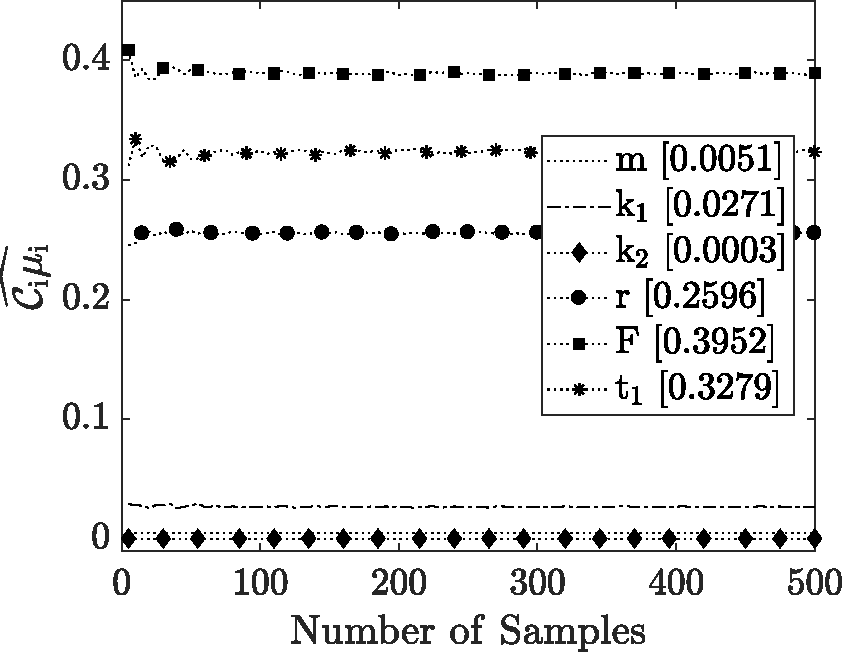
\includegraphics[width=0.48\textwidth]{./Figures/ub_conv_oscillator}
\caption{
Left: Sobol' total sensitivity index, $\mathcal{T}(\theta_i)$ for uncertain parameters in the limit 
state function in~\eqref{eq:limit}. Right: 
Estimates of the screening metric ($\widehat{\mathcal{C}_i\mu_i}$), plotted
against number of samples. Also included in the legend are estimates of $\mathcal{T}(\theta_i)$
in each case in the legend.}
\label{fig:sense_osc}
\end{center}
\end{figure}
We note that the total Sobol sensitivity indices are in excellent agreement
with the screening metric estimates. 
Consequently, the parameter ranks are found to be consistent in the
two plots in  
Figure~\ref{fig:sense_osc}.
It is observed that the limit state function is predominantly sensitive 
to $r$, $F$, and $t_1$. Hence, it seems likely that an ROS in
three dimensions is able to capture the overall uncertainty in $g(\bm{X})$.
% due to uncertainty in the six parameters. 
To illustrate computational gains as a
result of dimension-reduction, we construct PCEs in 3D, 4D (accounts for the
uncertainty in $k_1$ as well), and the original 6D parameter domain. In
Figure~\ref{fig:conv_osc}~(left), we compare the convergence of the
PCEs. As expected, the third-order PCE converges much faster than the other
two. Consequently, the number of model evaluations required for a converged PCE
is expected to be relatively much smaller in this case.  
\begin{figure}[htbp]
 \begin{center}
  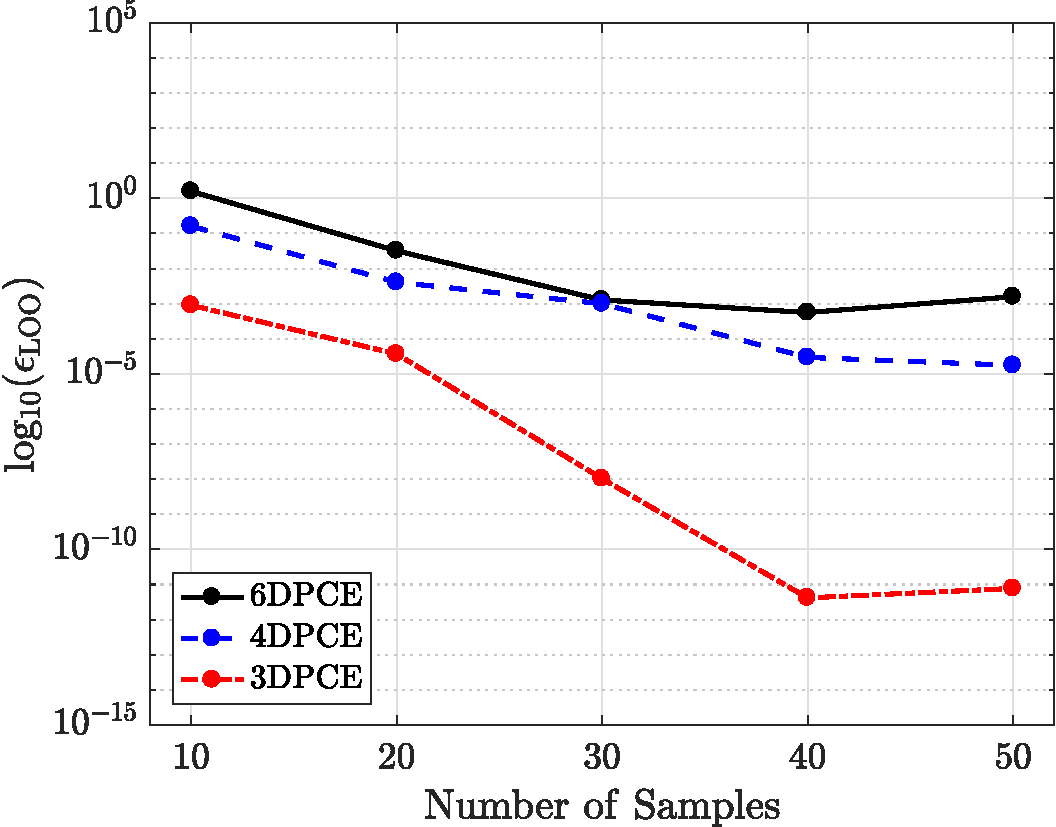
\includegraphics[width=0.48\textwidth]{./Figures/err_samples_oscillator}
  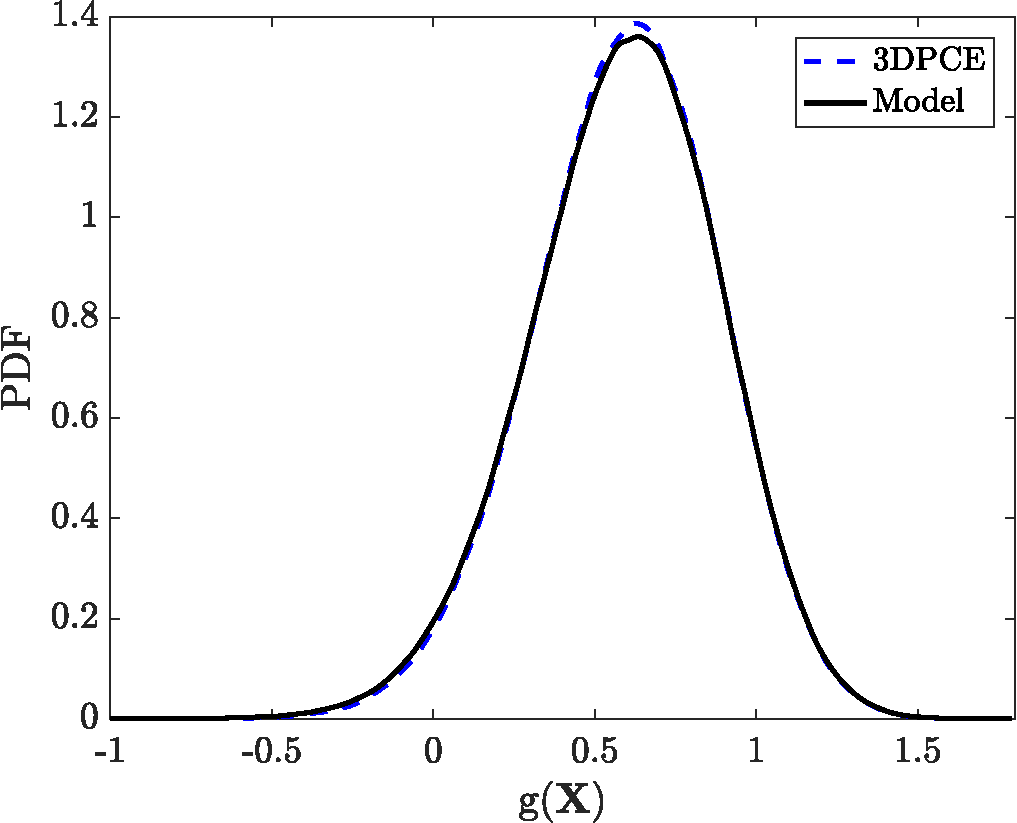
\includegraphics[width=0.48\textwidth]{./Figures/pdf_comp_oscillator}
\caption{Left: Logarithm of $\epsilon_{\mbox{\tiny{LOO}}}$ is plotted against sample size for 
PCEs constructed in 3, 5, and 6 dimensions to compare their convergence characteristics. 
Right: PDF of the limit state function is plotted using the actual function in~\eqref{eq:limit}
and the third-order PCE.}
\label{fig:conv_osc}
\end{center}
\end{figure}

To verify the accuracy of the third-order PCE, we estimate the relative L-2
norm of the difference between predictions of  $g(\bm{X})$, obtained using the
actual function in \eqref{eq:limit} and the 
PCE using \eqref{eq:l2}, and a validation test suite. The test suite comprised
model evaluations at 1000 independent Monte-Carlo samples in the full 
parameter space. The value of $\epsilon_{\mbox{\tiny{L-2}}}$ 
was found to be 0.0835 i.e. the third-order PCE is accurate within 8.36$\%$.
Furthermore, the accuracy is assessed in a probabilistic sense by comparing
in Figure~\ref{fig:conv_osc}~(right),
PDFs of $g(\bm{X})$, obtained using the full-surrogate, reduced-order 
surrogates constructed 3 and 4 dimensions, and a normalized histogram based
on model evaluation in the validation test suite. The three PDFs are observed
to be in excellent agreement with each other as well as the model-based
histogram. Hence, the ROS constructed using the methodology
presented in section~\ref{sec:method} could be used reliably to 
quantify the uncertainty in $g(\bm{X})$ with reduced effort.

\subsection{Semi-linear elliptic PDE with random source term}

We consider the following semi-linear elliptic PDE: 
\begin{equation}\label{eq:semilinear}
\begin{aligned}
-\kappa \Delta u + c u^3 &= q \quad \text{in } \Omega,\\
 u &= 0 \quad \text{on } \partial \Omega.
\end{aligned}
\end{equation}
Here $\Omega = (0, 1)\times(0,1)$, 
$u$ is the state variable, and $\kappa$ and $c$ are coefficients of the diffusion term
and the nonlinear term in the above equation respectively. 
We consider uncertainties in $\kappa$, $c$, and the source term. 
The right hand side function $q$ is defined by 
\be
q(x, y) = 
\sum\limits_{i=1}^{N=8}\alpha_i\sin\left(\frac{i\pi x}{8}\right)
                               \cos\left(\frac{i\pi y}{8}\right),
\label{eq:source}
\ee
where $\alpha_i$, $i = 1, \ldots, 8$ are random coefficients.
%
Hence, $u~=~u(\vec{\theta})$, where $\vec{\theta} = 
(\kappa,c,\alpha_1,\alpha_2,\ldots,\alpha_{8})^T$ is the vector
of uncertain parameters. Distributions of the uncertain
input parameters are tabulated in Figure~\ref{fig:elliptic}~(left).
The solution of~\eqref{eq:semilinear} for
a fixed set of values of the uncertain parameters is also 
illustrated.

\begin{figure}[htbp]
\begin{center}
\begin{minipage}[htbp]{.25\linewidth}
\vspace{0pt}
%\centering
\hspace{-25mm}
\begin{tabular}{cl}
\toprule
$\theta_i$ & \textbf{Distribution} \\ 
\bottomrule
$\kappa$ & $\mathcal{U}$[0.05,0.1] \\
$c$ & $\mathcal{U}$[1.0,2.0] \\
$\alpha_i$ & $\mathcal{U}$[0.0,4.0] \\
\bottomrule
\end{tabular}
\end{minipage}
\hspace{-20mm}
\begin{minipage}[htbp]{.25\linewidth}
\vspace{0pt}
%\centering
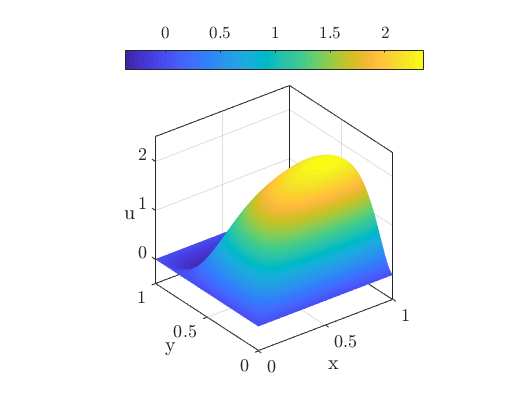
\includegraphics[width=3.0in]{./Figures/u_soln.png}
\end{minipage}%
\end{center} 
\caption{Left: Table providing distributions of the individual
uncertain parameters in~\eqref{eq:semilinear}. Right: Solution
of the 2D semilinear elliptic PDE~\eqref{eq:semilinear} using
$\kappa$~=~0.075, $c$~=~1.5, and $\alpha_i$~=~4.0}
\label{fig:elliptic}
\end{figure}

We aim to construct a reduced-order surrogate for the following QoI:
\be
\mathcal{F}(\kappa, c, \theta) = \frac{1}{|D|} \int_D u(x; \kappa, c, \theta) \, dx, 
\label{eq:qoi}
\ee
%
where $D$ is the region $[2/5, 3/5] \times [2/5, 3/5] \subset \Omega$, 
and $|D|$ denotes the area of $D$. 
While this model is considerably more complex than the previous numerical
examples, it can still be solved efficiently.
The equation was discretized using finite-differences, and Newton's method
was used to solve the resulting nonlinear system on a (100$\times$100) 2D
cartesian grid.~\alennote{Give the
number of degrees of freedom.} 
We computed converged estimates of the Sobol
total-effect index $\mathcal{T}(\theta_i)$, reported 
in Figure~\ref{fig:sense_elliptic}~(left) by solving the above non-linear
system at 500 samples in the 10D parameter space. 
%
\begin{figure}[htbp]
 \begin{center}
  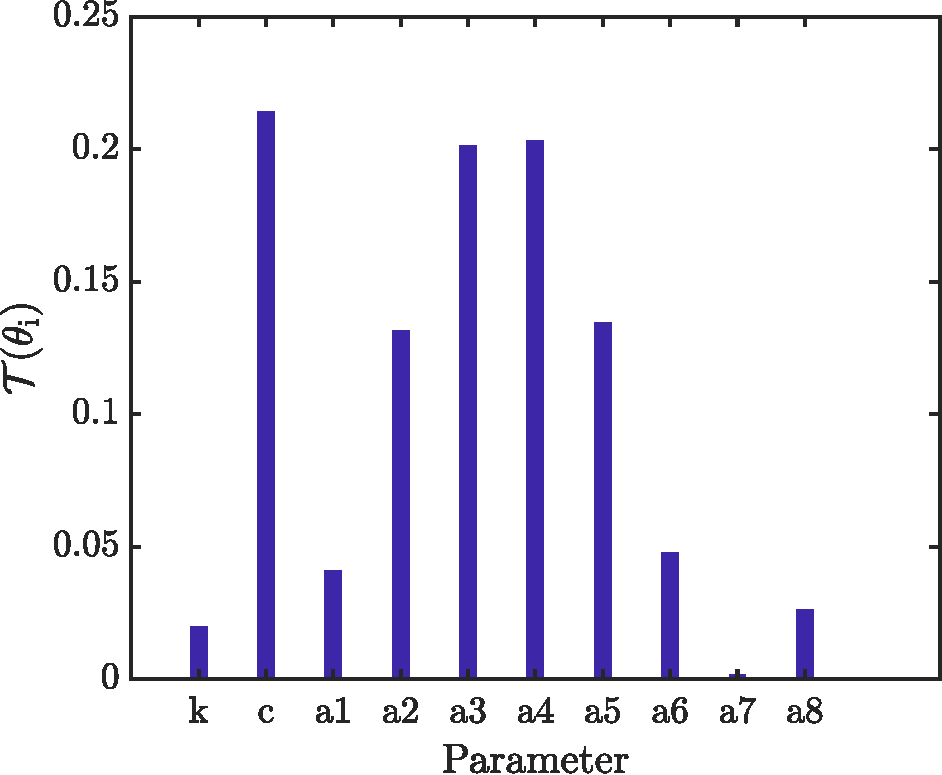
\includegraphics[width=0.46\textwidth]{./Figures/sense_elliptic}
  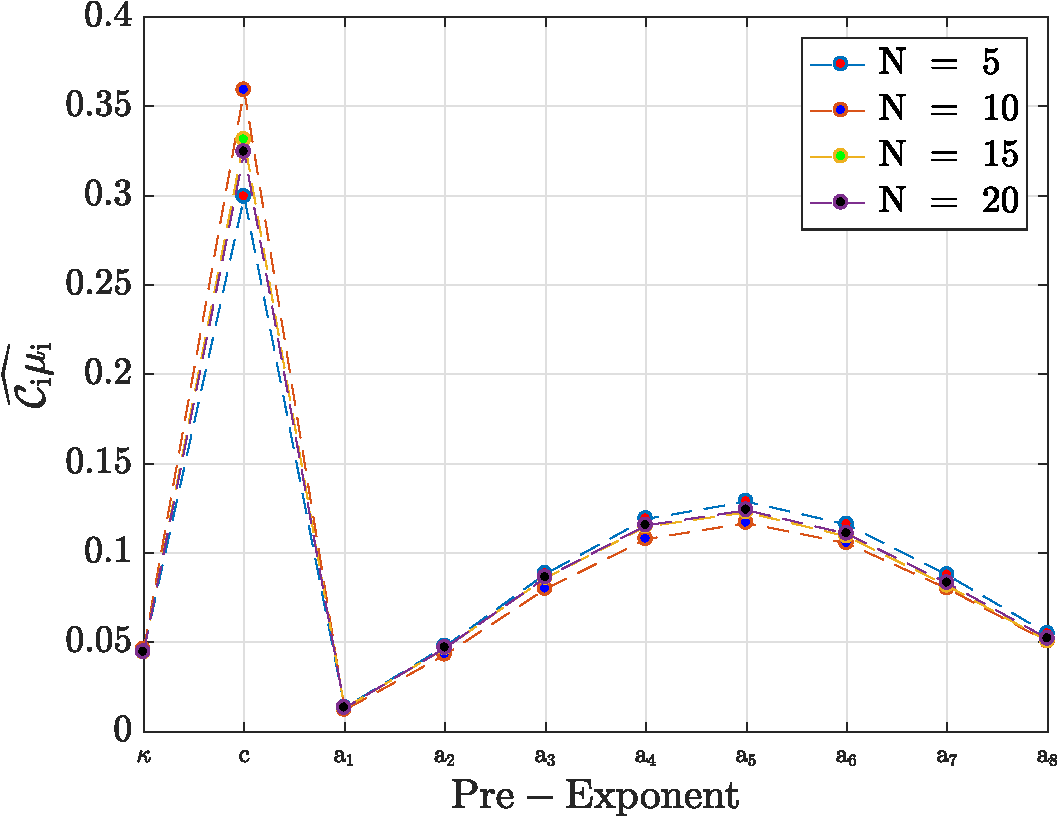
\includegraphics[width=0.48\textwidth]{./Figures/ub_conv_elliptic}
\caption{
Left: Sobol' total sensitivity index, $\mathcal{T}(\theta_i)$ for uncertain parameters in the 
semilinear elliptic PDE~\eqref{eq:semilinear}. Right: 
Estimates of the screening metric ($\widehat{\mathcal{C}_i\mu_i}$) for each uncertain parameter,
obtained using $N$ = 5, 10, 15, and 20 samples in the full parameter space.}
\label{fig:sense_elliptic}
\end{center}
\end{figure}
%
Sensitivity predictions based on the screening metric, $\widehat{\mathcal{C}_i\mu_i}$,
plotted in Figure~\ref{fig:sense_elliptic}~(right), are found to
be in close agreement with $\mathcal{T}(\theta_i)$, even for the case when $N$ = 5. As $N$
is increased from 5 to 20, estimates of the screening metric are observed to converge.
Based on the trends observed in Figure~\ref{fig:sense_elliptic}, it can be said that
the uncertainty in the QoI in \eqref{eq:qoi} is largely dependent on $c$, 
$\alpha_2$, $\alpha_3$, $\alpha_4$, and $\alpha_5$. These observations underscore the
potential for computational gains by constructing an ROS in the 5D parameter space. We 
illustrate the comparison of convergence characteristics of the PCEs constructed in the
full parameter space (10D) and the reduced space (5D) in Figure~\ref{fig:conv_elliptic} (left). 
As expected, the ROS converges considerably faster. Using model evaluations at 90
sample points, $\epsilon_{\mbox{\tiny{LOO}}}$ is found to be two orders of magnitude
smaller than that in the case of full-surrogate ($\mathcal{O}(10^{-4}$) versus
$\mathcal{O}(10^{-2}$)). 
Consequently, the computational effort for constructing the ROS in the present test problem
is expected to be much smaller. 
%
\begin{figure}[htbp]
 \begin{center}
  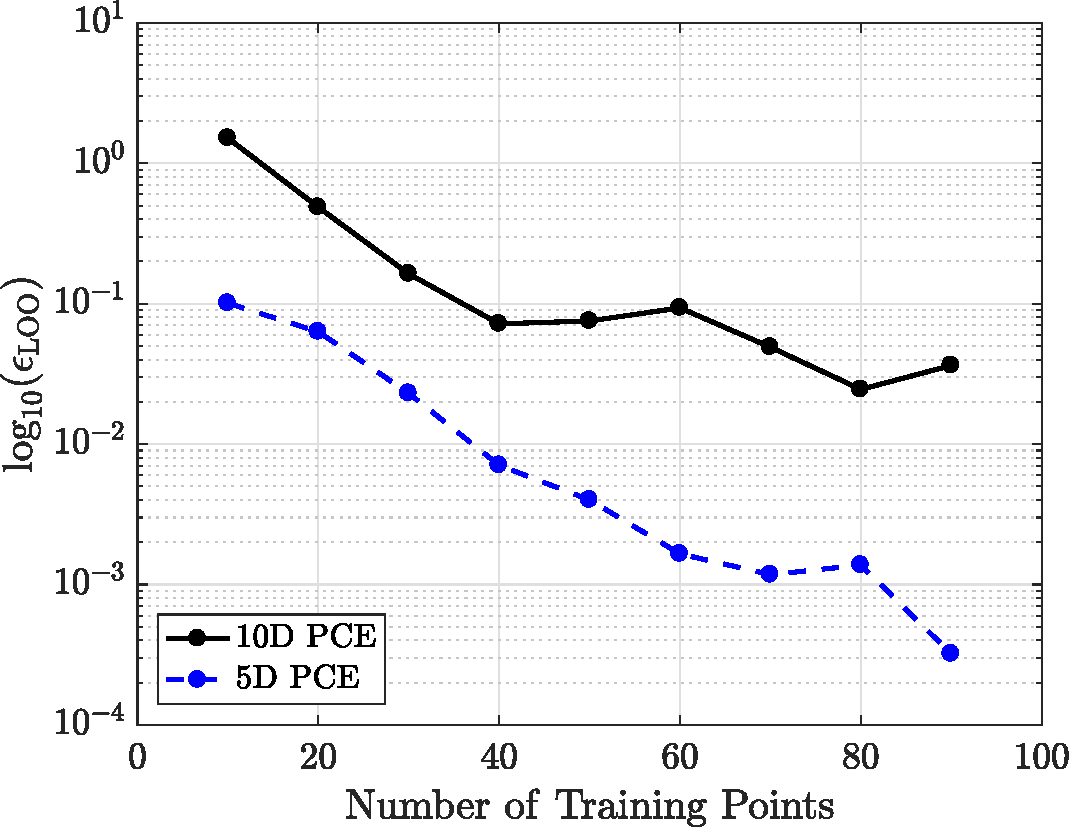
\includegraphics[width=0.48\textwidth]{./Figures/err_samples_elliptic}
  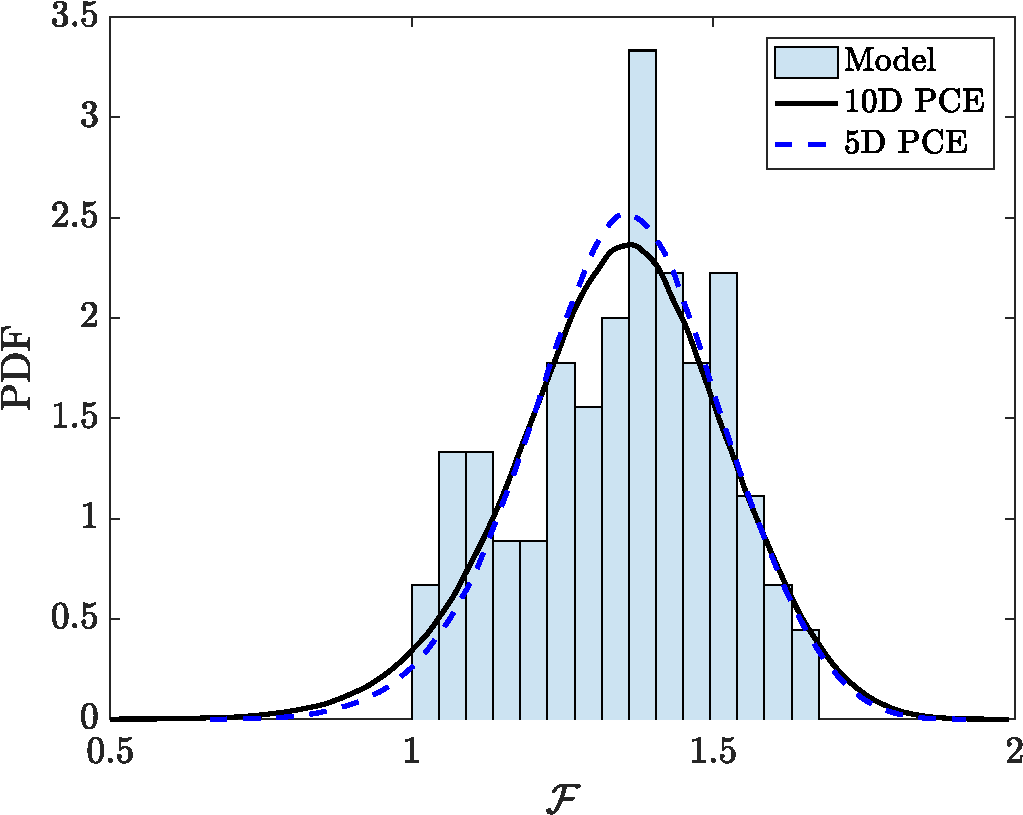
\includegraphics[width=0.48\textwidth]{./Figures/pdf_comp_elliptic}
\caption{Left: Logarithm of $\epsilon_{\mbox{\tiny{LOO}}}$ is plotted against sample size for 
PCEs constructed in 10 and 5 dimensions to compare their convergence characteristics. 
Right: PDF of the QoI, $\mathcal{F}(\kappa, c, \theta)$ in~\eqref{eq:semilinear} is
plotted using the full-surrogate and the reduced-order PC surrogate.}
\label{fig:conv_elliptic}
\end{center}
\end{figure}

Once again, we verify the accuracy of the ROS by estimating $\epsilon_{\mbox{\tiny{L-2}}}$
using model evaluations at 1000 independent Monte-Carlo samples in the 10D parameter
space. The ROS was found to be accurate
within 5$\%$. In order to bolster confidence in the ROS, we compare PDFs of the QoI
as well as a normalized histogram plot based on sparse model evaluations in the  
validation test-suite, in 
Figure~\ref{fig:conv_elliptic}~(right). While the two PDFs are in favorable agreement,
the modal estimate and the spread in the QoI based on the histogram is also captured
by them. Hence, the ROS could be used with a reasonable degree of confidence to
quantify the uncertainty in $\mathcal{F}(\kappa, c, \theta)$ thereby leading to
a computational advantage in this case.
































\bigskip
\bigskip


\section{Application: H$_2$/O$_2$ Reaction Kinetics}
\label{sec:app}

%Problem set-up: something about the reaction - why is it important?
%different reactions, reaction rate definition, uncertain parameters,
%quantity of interest. 
%
%Implementation of the proposed methodology for two scenarios: lean
%mix and rich mix. Describe what we mean by lean and rich using
%stoichiometry. 
%
%Define all the inputs as per the framework and illustrate its
%implementation to this application for both scenarios

The proposed framework in section~\ref{sec:method} is implemented to 
the H$_2$/O$_2$ reaction mechanism provided in~\cite{Yetter:1991}.
The H$_2$/O$_2$ reaction is gaining a lot of attention as a potential
source of clean energy for applications such as 
transportation~\cite{Das:1996} and fuel cell 
applications~\cite{Loges:2008,Cosnier:2016}. We begin by providing
the necessary background information for setting up the problem
in~\ref{sub:setup}. Results and discussion based on the implementation
of the proposed framework are provided in~\ref{sub:imp}. Finally, 
in~\ref{sub:cost}, we
provide a comparative analysis of the computational cost involved
in determining relative parameter importance using DGSMs and the
total-effect Sobol' index as the dimensionality increases from 19 to 33
for the present application.

\subsection{Problem Setup}
\label{sub:setup}  
The mechanism comprises of 19 reactions including chain reactions,
dissociation/recombination reactions, and formation and consumption
of intermediate species as provided below in Table~\ref{tab:kinetics}.
%
\begin{table}[htbp]
\renewcommand*{\arraystretch}{1.2}
\begin{center}
\begin{tabular}{llll}
\toprule
Reaction \#     & Reaction &&\\
\bottomrule
$\mathcal{R}_1$ & H + O$_2$          & $\rightleftharpoons$ & O + OH \\
$\mathcal{R}_2$ & O + H$_2$          & $\rightleftharpoons$ & H + OH \\
$\mathcal{R}_3$ & H$_2$ + OH         & $\rightleftharpoons$ & H$_2$O + H \\
$\mathcal{R}_4$ & OH + OH            & $\rightleftharpoons$ & O + H$_2$O \\
$\mathcal{R}_5$ & H$_2$ + M          & $\rightleftharpoons$ & H + H + M \\
$\mathcal{R}_6$ & O + O + M          & $\rightleftharpoons$ & O$_2$ + M \\
$\mathcal{R}_7$ & O + H + M          & $\rightleftharpoons$ & OH + M \\
$\mathcal{R}_8$ & H + OH +M          & $\rightleftharpoons$ & H$_2$O + M \\
$\mathcal{R}_9$ & H + O$_2$ + M      & $\rightleftharpoons$ & HO$_2$ + M \\
$\mathcal{R}_{10}$ & HO$_2$ + H      & $\rightleftharpoons$ & H$_2$ + O$_2$ \\
$\mathcal{R}_{11}$ & HO$_2$ + H      & $\rightleftharpoons$ & OH + OH \\
$\mathcal{R}_{12}$ & HO$_2$ + O      & $\rightleftharpoons$ & O$_2$ + OH \\
$\mathcal{R}_{13}$ & HO$_2$ + OH     & $\rightleftharpoons$ & H$_2$O + O$_2$ \\
$\mathcal{R}_{14}$ & HO$_2$ + HO$_2$ & $\rightleftharpoons$ & H$_2$O$_2$ + O$_2$ \\
$\mathcal{R}_{15}$ & H$_2$O$_2$ + M  & $\rightleftharpoons$ & OH + OH + M \\
$\mathcal{R}_{16}$ & H$_2$O$_2$ + H  & $\rightleftharpoons$ & H$_2$O + OH \\
$\mathcal{R}_{17}$ & H$_2$O$_2$ + H  & $\rightleftharpoons$ & HO$_2$ + H$_2$ \\
$\mathcal{R}_{18}$ & H$_2$O$_2$ + O  & $\rightleftharpoons$ & OH + HO$_2$ \\
$\mathcal{R}_{19}$ & H$_2$O$_2$ + OH & $\rightleftharpoons$ & HO$_2$ + H$_2$O \\
\bottomrule
\end{tabular}
\end{center}
\caption{Reaction mechanism for H$_2$/O$_2$ from~\cite{Yetter:1991}}.
\label{tab:kinetics}
\end{table}
%
The reaction rate for the $i^{th}$ reaction as a function of temperature
is given as follows:
\be
k_i(T) = A_iT^{n_i}\exp(-E_{a,i}/RT), 
\label{eq:rate}
\ee
%
where $A_i$, $n_i$, and $E_{a,i}$ denote the pre-exponent, the index of $T$, and
and the activation energy corresponding to the $i^{th}$ reaction; and $R$ is the
universal gas constant. 
The TChem~\cite{Safta:2011} software package is used to model homogeneous
ignition at constant pressure for a range of initial conditions for the
fuel-oxidizer mixture. During the simulation, the fuel-oxidizer mixture goes 
through a radical build-up phase followed by a sharp increase in temperature
as heat is released during the thermal runaway. We focus on quantifying the 
uncertainty in the \emph{ignition delay} due to uncertainty associated 
with the pre-exponent, $A_i$, for each reaction. The ignition delay 
is defined as the inflection point on the temperature profile during the thermal
runaway. The total number of uncertain parameters in the
present case is 19.  The $A_i$'s are considered to be uniformly distributed in
the interval: $[0.9A_i^\ast, 1.1A_i^\ast]$; $A_i^\ast$ being the nominal
estimate corresponding to the $i^{th}$ reaction.
The set of nominal values used in the computations, for parameters 
in~\eqref{eq:rate} are provided
in~\cite{Yetter:1991}. 

While the dimensionality of the problem is moderate,
constructing a surrogate in the 19-dimensional parameter space could still be
expensive. Hence, we explore the possibility of constructing a
reduced-space surrogate (RSS) using the framework presented 
in section~\ref{sec:method}. 
In the present study, we focus on two scenarios: fuel(H$_2$)-rich, and
fuel(H$_2$)-lean. Consider the global reaction:
%
\be
2\text{H}_2 + \text{O}_2 \rightarrow 2\text{H}_2\text{O}
\label{eq:global}
\ee 
%
The equivalence ratio $\phi$ is defined as follows:
%
\be
\phi = \frac{(M_{\text{H}_2}/M_{\text{O}_2})_\text{obs}}{(M_{\text{H}_2}/M_{\text{O}_2})_\text{st}}
\label{eq:phi}
\ee
%
The numerator in the right-hand-side represents the observed (obs) fuel-oxygen
mass ratio at a given condition and the denominator represents the
stoichiometric (st) ratio of the same quantity. Hence, $\phi$ = 1 at
stoichiometric conditions. The equivalence ratio can be altered by changing the
amount of O$_2$ in the mixture. In the case of a lean
mixture,~\eqref{eq:global} can be written as follows:
%
\be
2\text{H}_2 + \alpha\text{O}_2 \rightarrow 2\text{H}_2\text{O} + (\alpha-1)\text{O}_2 
\hspace{3mm} (\alpha>1)
\label{eq:lean}
\ee 
%
Similarly, for the case when the mixture if fuel rich,~\eqref{eq:global} is modified
as follows:
%
\be
2\text{H}_2 + \alpha\text{O}_2 \rightarrow 2\alpha\text{H}_2\text{O} + 2(1-\alpha)\text{H}_2
\hspace{3mm} (\alpha<1)
\label{eq:rich}
\ee 
%
Eqs.~\eqref{eq:lean} and~\eqref{eq:rich} can be generalized as follows:
%
\be
2\text{H}_2 + \alpha\text{O}_2 \rightarrow 2\min(1,\alpha)\text{H}_2\text{O} + 
\max(\alpha-1,0)\text{O}_2 + \max(0,2-2\alpha)\text{H}_2
\label{eq:gen}
\ee 
%
From the above set of chemical equations, the relationship between $\phi$
and $\alpha$ can be easily obtained as $\phi~=~\frac{1}{\alpha}$.
Since $\phi>1$ corresponds to a rich mixture, and $\phi<1$ corresponds to a
lean mixture, we consider $\phi$ = 2.0 and 0.5 to investigate the two scenarios
respectively. 

\subsection{DGSM-guided surrogate construction}
\label{sub:imp}
We apply the parameter screening algorithm with the following
parameters: $\tau_\text{screen}$, $s_\text{min}$,
$s_\text{max}$, $\beta$ are fixed at 0.2, 3, 10, and 1.0 respectively for both cases.
Additionally, the value of $\tau$ is considered to be 1.0$\times 10^{-17}$ and
5.0$\times 10^{-17}$ in the rich and lean case respectively. Such a small value
of $\tau$ for this application is a consequence of the nature of convergence exhibited
by the sensitivity measures. Moreover, the screening procedure is carried out
for atleast $s_\text{min}$ number of iterations in order to bolster our confidence
in the estimates. 

Following the steps outlined in the flow-diagram in Figure~\ref{fig:flow}, model
evaluations are initially generated at $n_1$ = 5 samples. The evaluations are
used to construct a regression-based surrogate in the full-space. As
expected, the surrogate is found to be highly inaccurate. Moreover, unlike the
test problems in section~\ref{sec:examples}, we do not estimate the Sobol'
total-effect sensitivity indices in the interest of following the overall framework
closely. Hence, we proceed to the screening step to estimate the screening metric
for the uncertain pre-exponents, $A_i$'s. Results are plotted below
in Figure~\ref{fig:sense_kinetics}~(top row) for both cases. Furthermore, we illustrate
the decay in the value of $\Delta\mu_s$ with iterations in 
Figure~\ref{fig:sense_kinetics}~(bottom row). 

\begin{figure}[htbp]
 \begin{center}
  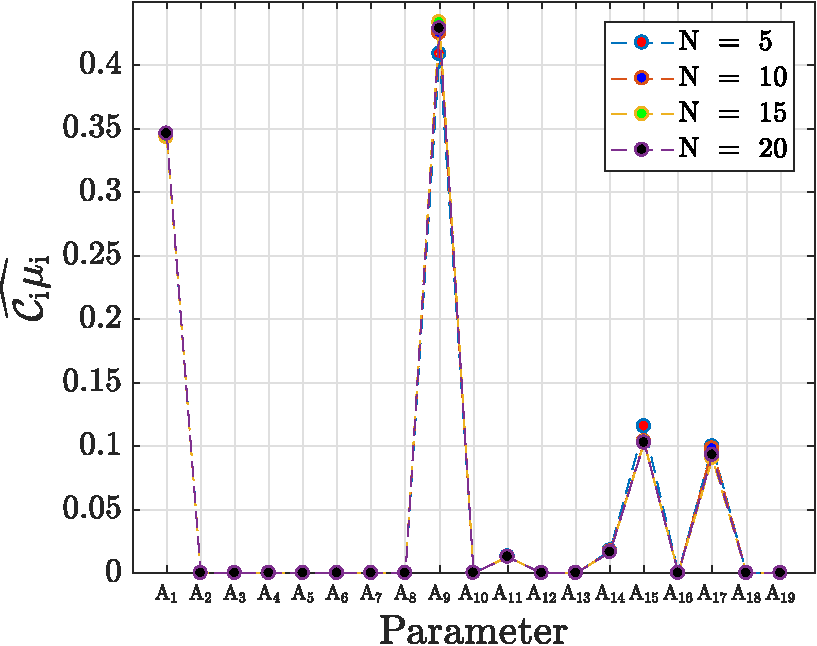
\includegraphics[width=0.45\textwidth]{./Figures/ub_conv_kinetics_rich}
  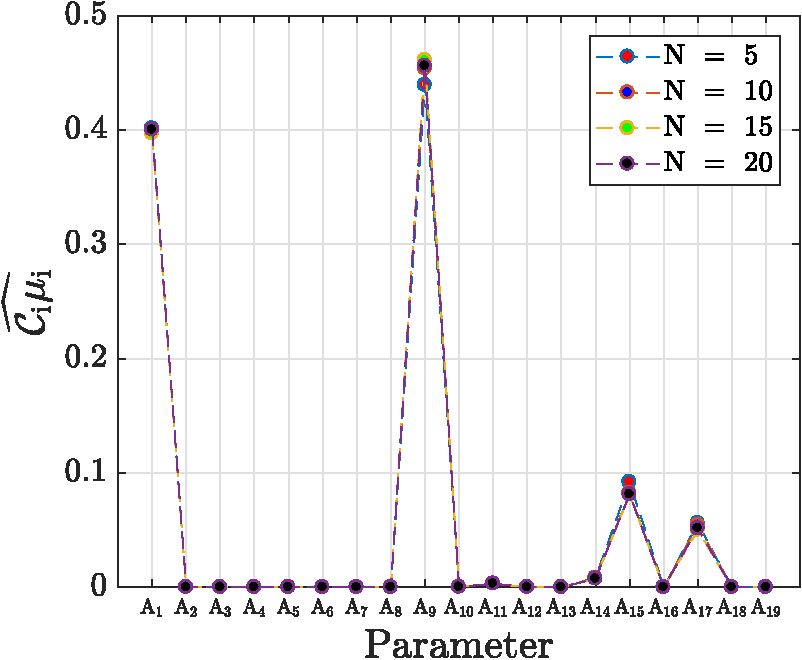
\includegraphics[width=0.45\textwidth]{./Figures/ub_conv_kinetics_lean}
  \\ \vspace{2mm}
  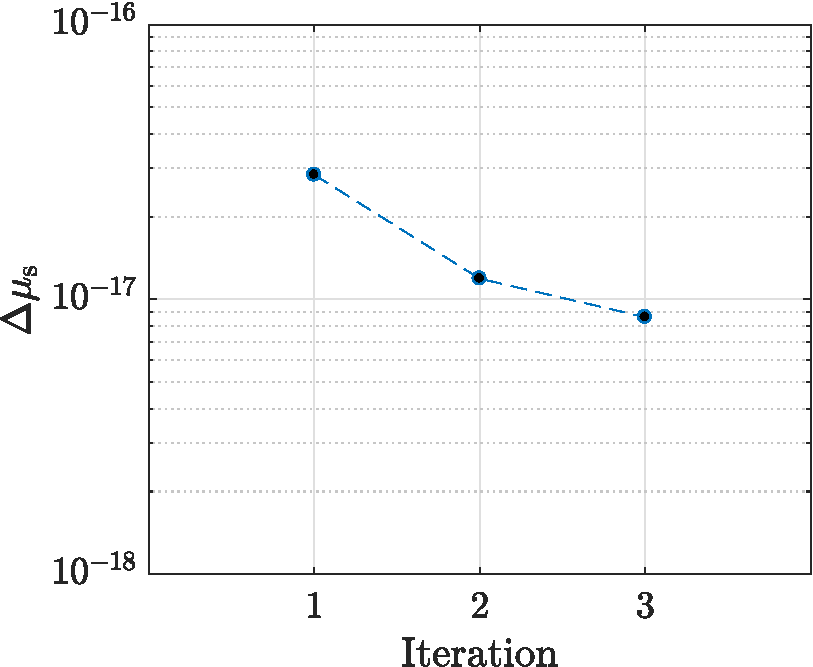
\includegraphics[width=0.45\textwidth]{./Figures/mu_rich}
  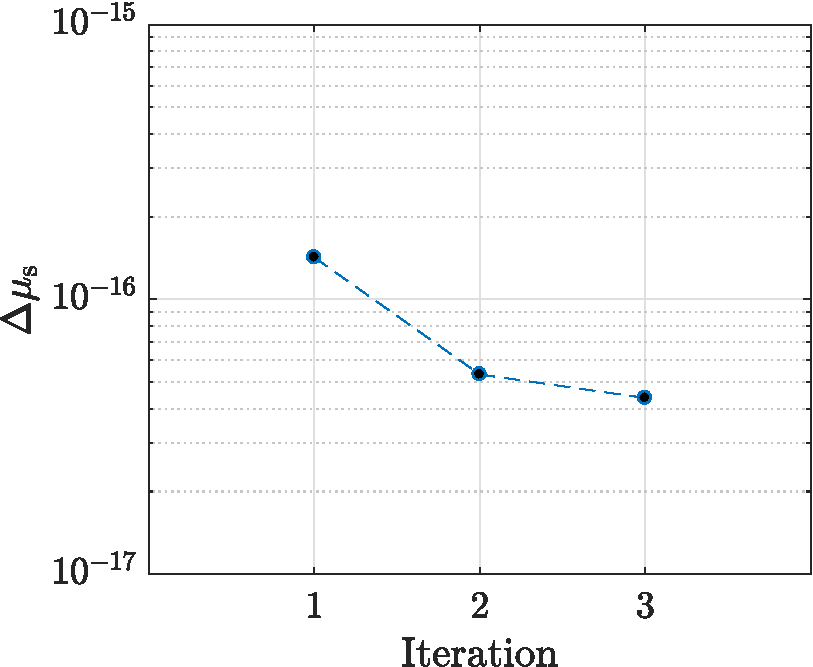
\includegraphics[width=0.45\textwidth]{./Figures/mu_lean}
\caption{Top: Estimates of $\widehat{\mathcal{C}_i\mu_i}$ for $A_i$'s in the case
of fuel-rich mixture~(left) and fuel-lean mixture~(right). Bottom: The value of
$\Delta\mu_s$ during three iterations within the screening step are plotted for
the case of fuel-rich mixture~(left) and fuel-lean mixture~(right).}
\label{fig:sense_kinetics}
\end{center}
\end{figure}
%
The screening metric estimates in the above plots are observed to converge with
only a few samples (5--10). Moreover, out of the 19 uncertain pre-exponents,
only $A_1$, $A_9$, $A_{15}$, and $A_{17}$ seem to be important in the fuel-rich
case, whereas, only $A_1$, $A_9$, and $A_{15}$ seem important in the fuel-lean
case, based on the value of $\tau_\text{screen}$. These observations are indicative
of the potential for significant reduction in the dimensionality of this problem. 
A reduced-space
surrogate constructed using the proposed framework could thus lead to large computational
gains. The decay of $\Delta\mu_s$ with iterations is expected and builds our confidence
in the screening procedure in both cases.

A reduced-space surrogate (RSS) was constructed in 4D for the fuel-rich case,
and in 3D for
the fuel-lean case. Figure~\ref{fig:err_samples_kinetics}~(left) illustrates a
comparison of convergence characteristics for the PCEs constructed in the
full-space and the reduced-space for the fuel-rich case. Note that the
plot is generated using the implementation of least angle regression (LAR)
for sparse PCEs in UQLab.  
%
\begin{figure}[htbp]
 \begin{center}
  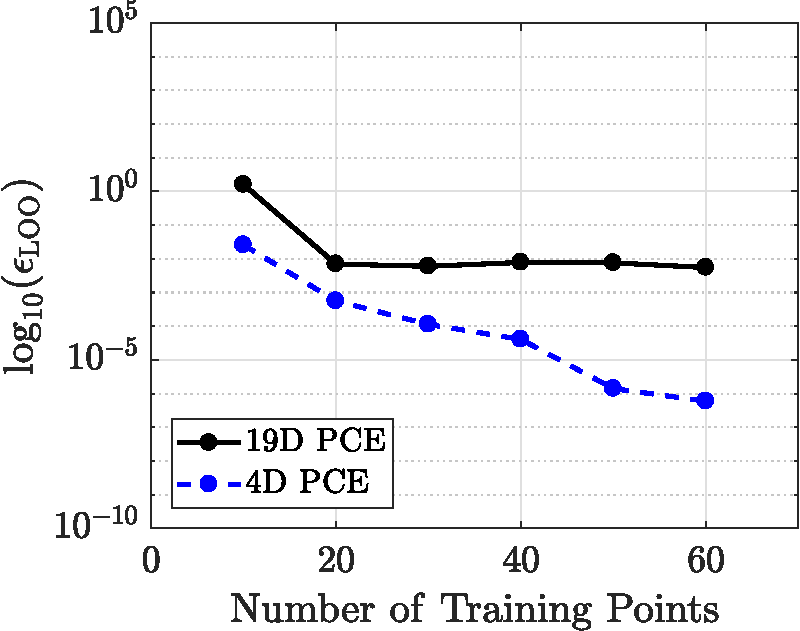
\includegraphics[width=0.45\textwidth]{./Figures/err_samples_kinetics}
   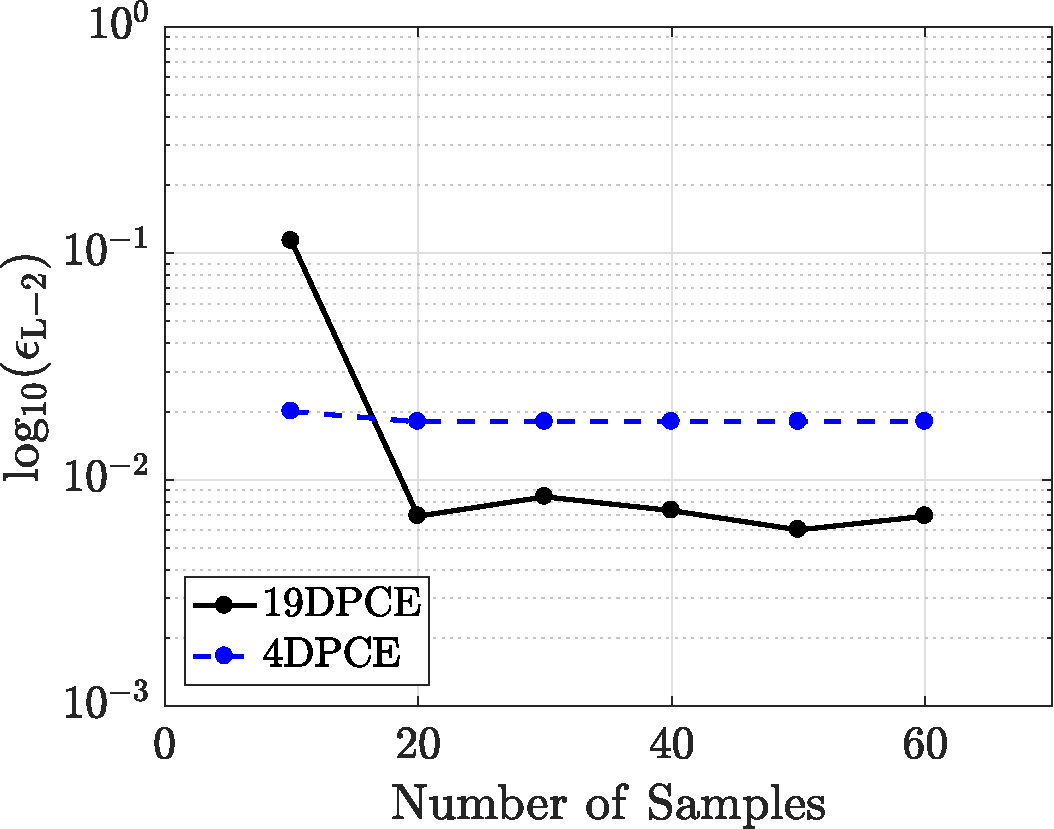
\includegraphics[width=0.44\textwidth]{./Figures/errL2_samples_kinetics}
\caption{Left: A semi-log plot of $\epsilon_\text{\tiny LOO}$ as a function of
number of model evaluations in the full-space (19D) and the reduced-space (4D)
for the fuel (H$_2$)-rich case i.e. $\phi$ = 2.0. The degree of
the PCE constructed using 60 training points was found to be 1 and 3 in the 19D and the 4D cases respectively.
Right: Semilog plot of the relative L-2 error norm ($\epsilon_{\mbox{\tiny{L-2}}}$)
for the PCEs constructed in 4D and 19D.}
\label{fig:err_samples_kinetics}
\end{center}
\end{figure}
%
The leave-one-out cross validation error is observed to drop initially
and plateau with the increase in training points for the 19-dimensional
PCE. However, in the case of 4-dimensional PCE, the error exhibits a
monotonic behavior and is found to be smaller than $\mathcal{O}(10^{-5})$
at 60 training points. Clearly, the RSS shows a much faster rate of convergence.
Additionally, the
convergence of the relative error norm, $\epsilon_{\mbox{\tiny{L-2}}}$ in 
Figure~\ref{fig:err_samples_kinetics}~(right) indicates that for the case of 10
samples, the 4D PCE is observed to be more accurate. However, the 19D PCE
is observed to be more accurate by an order of magnitude as the sample size
increases. Specifically, the 4D PCE was found to be accurate within 1.8$\%$ in the
fuel-rich case, and within 3.1$\%$ in the fuel-lean case. Therefore, the 4D PCE
is still observed to be reasonably accurate in this case. Moreover, its faster convergence
as mentioned earlier should help reduce computational effort associated with
surrogate model construction.
Similar trends (not included) were observed in the fuel-lean case. 

Model evaluations at 1000 samples in the test suite
are further used to plot a normalized histogram of the ignition time in 
Figure~\ref{fig:pdf_kinetics}. To verify the accuracy of the RSS in a 
probabilistic-sense, we compare the histogram plot with a PDF of ignition time
using surrogate predictions at 10$^{6}$ samples in the reduced space in both cases. 
%
\begin{figure}[htbp]
 \begin{center}
  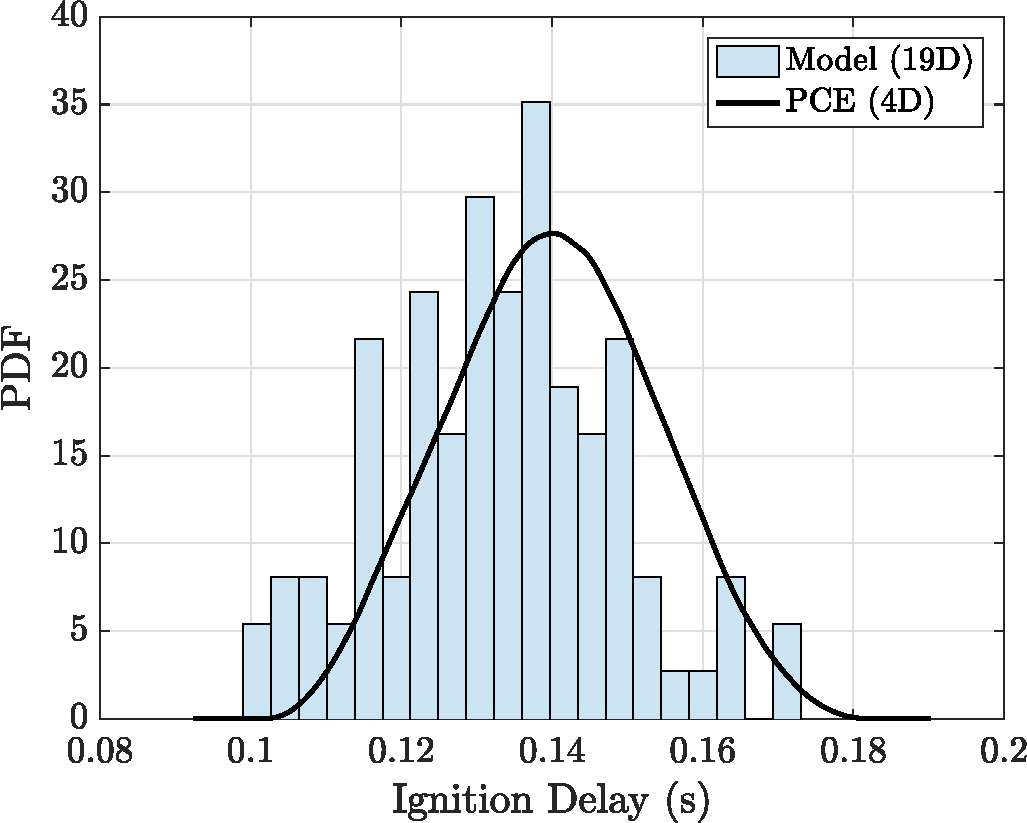
\includegraphics[width=0.45\textwidth]{./Figures/pdf_comp_rich}
  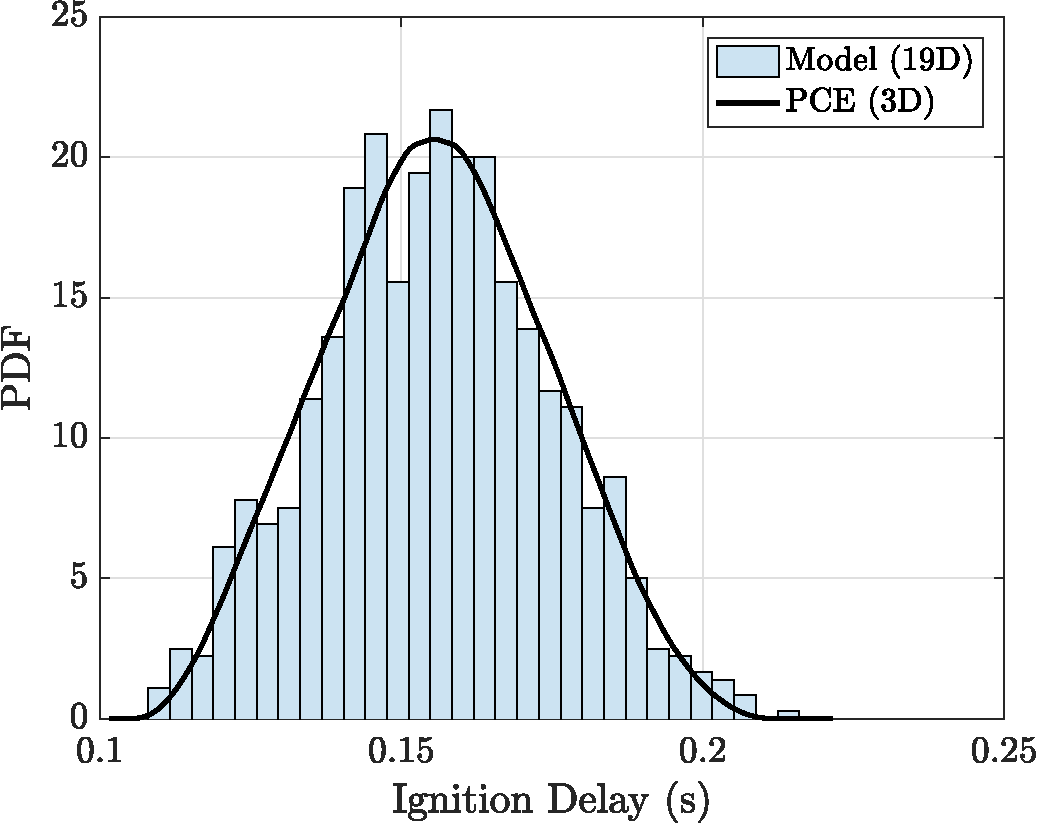
\includegraphics[width=0.45\textwidth]{./Figures/pdf_comp_lean}
\caption{A normalized histogram based on model evaluations at 1000 samples is plotted
along with a PDF of ignition delay for the fuel-rich case (left) and the fuel-lean
case (right).}
\label{fig:pdf_kinetics}
\end{center}
\end{figure}
%
Clearly, the RSS captures the spread as well as the modal estimate of
the ignition delay in both scenarios. Hence, the proposed framework 
has enabled significant dimension reduction and construction of an accurate
RSS for multiple scenarios pertaining to the H$_2$/O$_2$ reaction
mechanism.    


\subsection{Comparative cost analysis: higher-dimensional setting}
\label{sub:cost}

In this section, we perform a comparative analysis of the computational cost
associated with obtaining converged estimates of parametric sensitivities
using DGSM, and the total-effect Sobol' indices ($\mathcal{T}(\theta_i)$). The former is computed
using the parameter screening algorithm (Algorithm~\ref{alg:screen}), and the latter is
estimated using a sparse-basis PCE. Note that estimating $\mathcal{T}(\theta_i)$
using a PCE has been shown to be more efficient compared to sampling 
techniques~\cite{Crestaux:2009,BlatmanSudret10}.
Moreover, a sparse-basis PCE requires fewer training points which
enhances computational savings~\cite{Sudret:2008,Blatman:2009}. 
To investigate the impact of the dimensionality, the
analysis is performed with 19 uncertain parameters, i.e.
the pre-exponents~($A_i$'s) as discussed earlier in~\ref{sub:setup} and~\ref{sub:imp}, and
33 uncertain parameters wherein the activation energies~($E_{a,i}$'s) are considered to
be uncertain in addition to the $A_i$'s. The $E_{a,i}$'s are also considered to be uniformly distributed in the
interval: [$0.9E_{a,i}^\ast,1.1E_{a,i}^\ast$], where $E_{a,i}^\ast$ is the nominal value
for the $i^\text{th}$ reaction as provided in~\cite{Yetter:1991}. Note that only those
$E_{a,i}$'s with a non-zero nominal value are considered as uncertain, and therefore the
total number of uncertain parameters in the high-dimensional case is 33 as opposed to 38. 

The 33-dimensional sparse basis PCE was assessed for its convergence characteristics
and its predictive accuracy using $\epsilon_{\mbox{\tiny LOO}}$~(see~\eqref{eq:loo}) and
$\epsilon_{\mbox{\tiny{L-2}}}$~(see~\eqref{eq:l2}) respectively as shown in
Figure~\ref{fig:err_samples}.  
%
\begin{figure}[htbp]
 \begin{center}
  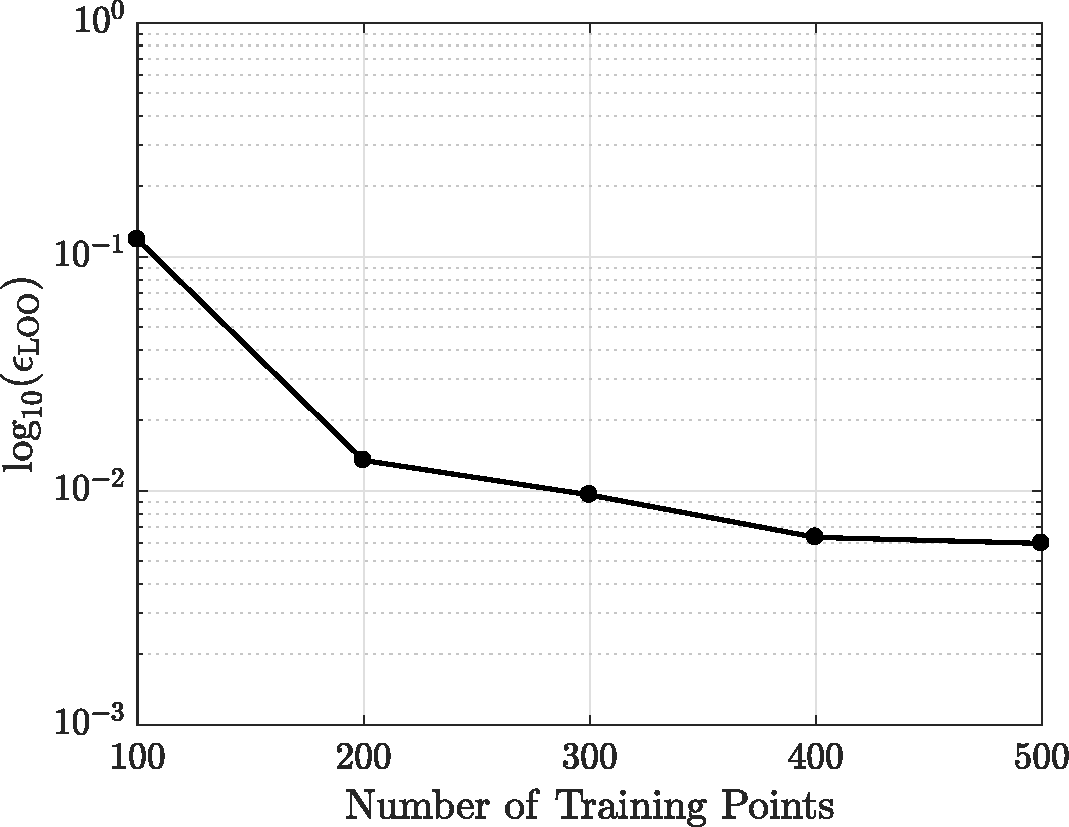
\includegraphics[width=0.45\textwidth]{./Figures/err_samples_kinetics33D}
\caption{A semi-log plot of $\epsilon_\text{\tiny LOO}$  and $\epsilon_{\mbox{\tiny{L-2}}}$
as a function of the number of training points in the 33D parameter space 
for the fuel (H$_2$)-rich case i.e. $\phi$ = 2.0. The degree of
the PCE constructed using 500 training points was found to be 3.}
\label{fig:err_samples}
\end{center}
\end{figure}
%
The sparse-basis PCEs constructed in the 19 and the 33 dimensional parameter
space were considered to have converged once $\epsilon_\text{\tiny LOO}$ was found to be
smaller than 6.0$\times$10$^{-3}$. As observed in Figures~\ref{fig:err_samples_kinetics}
and~\ref{fig:err_samples}, the number of training points required in the 19D
and the 33D cases are found to be 20 and 500 respectively. As expected, the predictive
accuracy is observed to increase with increase in the number of training points in both cases.
The estimate of $\epsilon_{\mbox{\tiny{L-2}}}$ was found to be 7.22$\times$10$^{-2}$ using the
converged 33D PCE and an independent set of model evaluations at 1000 samples.

Before comparing the computational cost pertaining to the two approaches (DGSM-based and 
Sobol'-based) and the impact of dimensionality, we verify that the parametric sensitivities are
consistent in both cases. Sensitivity estimates for the 33 uncertain parameters obtained
using the DGSM-based strategy, and by evaluating $\mathcal{T}(\theta_i)$ 
using the sparse-basis PCE are plotted and placed adjacent to each other for comparison
in Figure~\ref{fig:sense33D}.
%
\begin{figure}[htbp]
 \begin{center}
  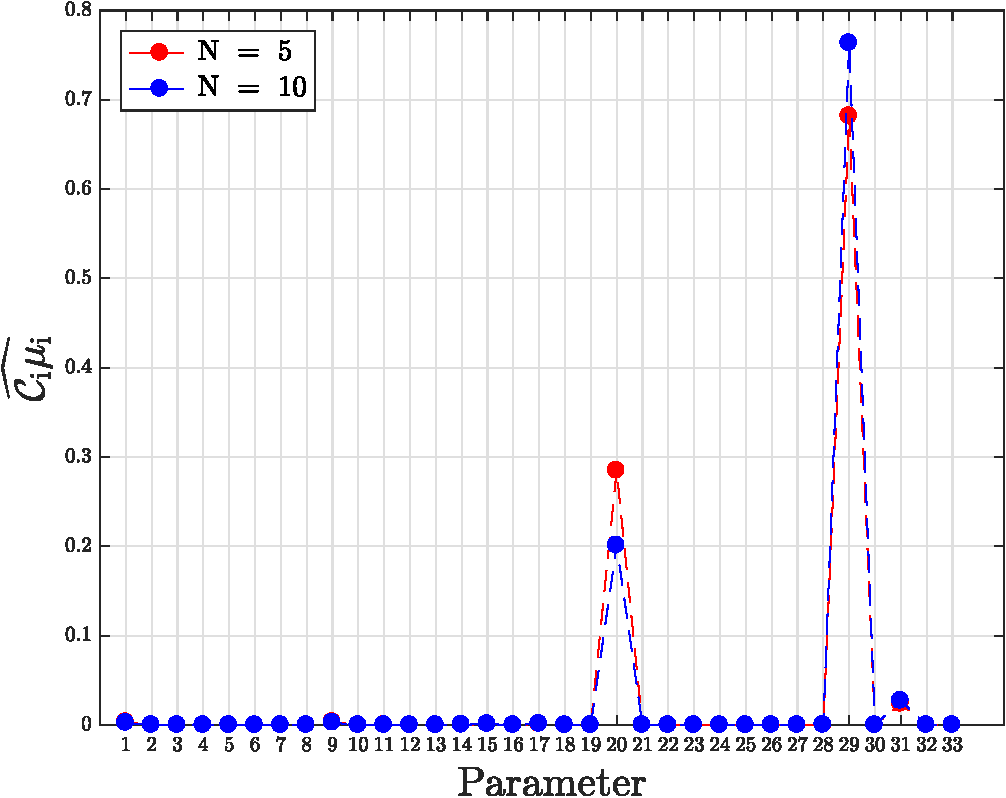
\includegraphics[width=0.42\textwidth]{./Figures/ub33D}
  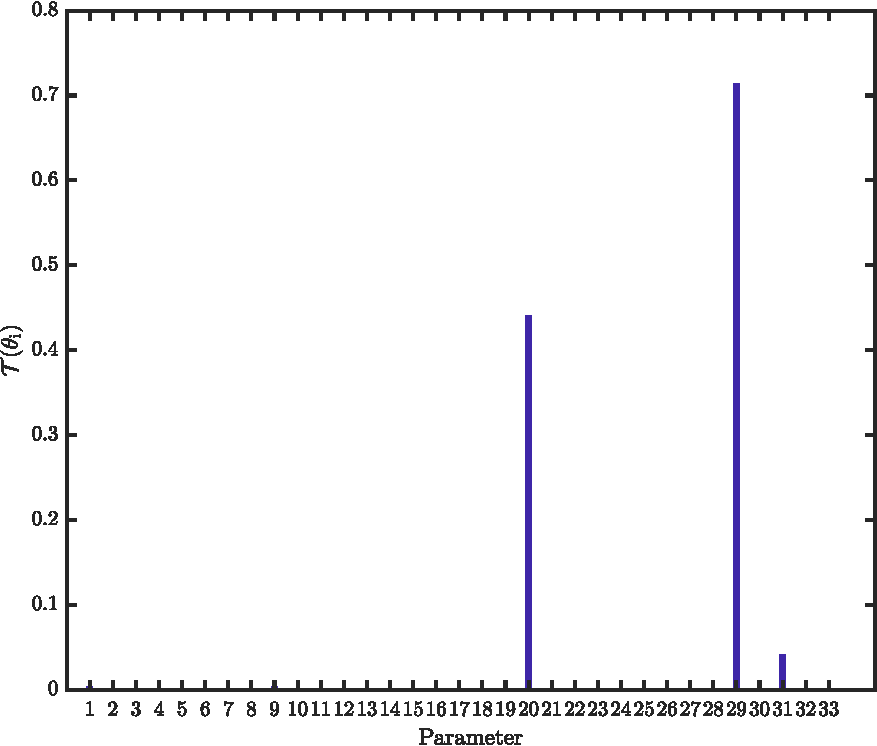
\includegraphics[width=0.40\textwidth]{./Figures/sens_kinetics33D}
\caption{
Left: Estimates of the screening metric ($\widehat{\mathcal{C}_i\mu_i}$), 
obtained using $N$ = 5, 10 samples in the full parameter space; and
Right: Total-effect Sobol' indices, $\mathcal{T}(\theta_i)$ for the 33 uncertain rate-controlling
parameters ($A_i$'s and $E_{a,i}$'s).}
\label{fig:sense33D}
\end{center}
\end{figure}
%
The plots clearly indicate that the relative importance of the uncertain parameters is
consistent in both cases. Specifically, both approaches reveal that the uncertainty in
the ignition delay is predominantly due to the uncertainty in $E_{a,1}$ and $E_{a,10}$ with a 
minor contribution from $E_{a,12}$, whereas, contributions from other parameters is either zero
or negligible. These results are clearly indicative of the potential for dimension reduction in this
case using the proposed sensitivity-driven approach. A reasonably accurate RSS in a 2D
parameter space could potentially capture the uncertainty in the ignition delay due to the
uncertainty in the 33 rate-controlling parameters.

The computational cost is estimated in terms of the number of function evaluations or model runs,
denoted by $\mathcal{M}$ in each case. In the case of DGSM-based approach presented in this work, 
$\mathcal{M}$ = $N(N_p+1)$ ($N$: number of samples, $N_p$: number of parameters)
as discussed earlier in~\ref{sub:dgsm}. In the case of PCE-based computation of $\mathcal{T}(\theta_i)$,
$\mathcal{M}$ is the sum total of the number of training points used for constructing the sparse-basis
PCE and the number of evaluations used for its verification. In Table~\ref{tab:cost},
we provide a comparison of $\mathcal{M}$ for the two approaches in the case of 19 and 33 uncertain
parameters for the H$_2$/O$_2$ reaction kinetics application. 
%
\begin{table}[htbp]
\renewcommand{\arraystretch}{1.5}
\caption{A comparison of computational cost for the DGSM-based and Sobol'-based parametric 
sensitivity analysis in the case of 19 and 33 uncertain rate-controlling parameters.}
\begin{center}
\begin{tabular}{c|p{4.2cm}|p{4.2cm}|}
\cline{2-3}
& \multicolumn{2}{ c| }{$\mathbf{\#}$ \textbf{of Function Evaluations/Model Runs}~($\mathcal{M}$)} \\ \cline{2-3} 
& \centering \textbf{19D} & \hspace{18mm} \textbf{33D} \\  \hhline{===}
\multicolumn{1}{ |l|| }{$\widehat{\mathcal{C}_i\mu_i}$ (\textbf{DGSM-based)}} & \centering 5(19+1) = 100 + $N_{v_1}$ & \hspace{3mm} 5(33+1) = 170 + $N_{v_1}$ \\ 
\cline{1-3}
\multicolumn{1}{ |l|| }{$\mathcal{T}(\theta_i)$ (\textbf{PCE-based})} & \centering 20 + $N_{v_2}$ & 
\hspace{13mm} 500 + $N_{v_2}$ \\ \cline{1-3}  
\end{tabular}
\end{center}
\label{tab:cost}
\end{table}
%
For the 19D case, estimating the converged estimates of the screening metric ($\widehat{\mathcal{C}_i\mu_i}$)
required 5 samples. However, since finite difference was used in this work for estimating the gradient of the
model output, a total of 100 model runs were required. Additionally, the screening procedure is continued for
one iteration using $N$ = 10 samples to ensure the convergence of $\widehat{\mathcal{C}_i\mu_i}$.
Since these additional runs are essentially used for verification, we denote them as $N_{v_1}$.
%As mentioned earlier in~\ref{sub:dgsm}, depending
%upon the application, it is possible to explore efficient techniques for gradient estimation such as those involving 
%adjoint computation and automatic differentiation. Hence, there is scope for a significant
%reduction in the computational cost
%associated with the DGSM-based approach. 
On the other hand, constructing the sparse-basis PCE requires only 20 samples in
the 19D parameter space with uncertain pre-exponents. Additional model runs ($N_{v_2}$)
 typically ranging from
$\mathcal{O}(10^{2})$ - $\mathcal{O}(10^{3})$ are needed to build a cross validation test suite to verify the 
accuracy of the PCE.  
The DGSM-based approach could thus yield computational gains especially when 
efficient gradient computation techniques are used. The comparison is significantly more favorable for the 
proposed DGSM-based framework in the higher dimensional case involving 33 uncertain parameters. 
Once again, converged estimates of the screening metric ($\widehat{\mathcal{C}_i\mu_i}$) are obtained
using only 5 samples in the 33D parameter space. For verification, the screening procedure is
continued for one iteration by evaluating the model output at 10 samples in 33 dimensions. 
Therefore, a total of 340 model runs are needed in this case
including for gradient computation using finite difference as well as verification. Whereas, as discussed earlier,
constructing the sparse PCE itself requires model runs at 500 training points to sufficiently converge. Additional
model runs ($\mathcal{O}(10^{2})$ - $\mathcal{O}(10^{3})$) are required to further verify the accuracy of the 
resulting PCE. Note that the analysis was performed
for the fuel-rich case. 

Based on our findings, it appears that the proposed DGSM-based approach can offer a significant
computational advantage especially in higher dimensions due to multiple factors: (1) Computational
effort required for estimating $\mathcal{T}(\theta_i)$ is observed to increase substantially with dimensionality even
when using sparse-basis PCEs. Whereas, the DGSM-based estimates converge
with only a few samples, $\mathcal{O}(10^1)$ even for a relatively higher-dimensional case. Moreover, it must be noted that
the computational gains associated with the proposed DGSM-based approach could be enhanced
significantly by employing efficient gradient computation techniques such as those involving adjoints
and automatic differentiation as mentioned earlier in~\ref{sub:dgsm}; (2) The number of model runs
needed to verify the convergence of $\widehat{\mathcal{C}_i\mu_i}$ can be controlled
using the iterative strategy in this work
and is expected to be much smaller than the number of runs needed for verifying the accuracy of  
$\mathcal{T}(\theta_i)$ especially in high-dimensional settings. Specifically, for the 33D case,
model runs at 5 additional samples (corresponding to the first iteration) were used to verify the
convergence of $\widehat{\mathcal{C}_i\mu_i}$ as opposed to 1000 model evaluations used to verify
the accuracy of the PCE. 
It can thus be understood that for higher dimensional problems involving hundreds of 
parameters, conventional approaches (even sparse-basis PCEs) can quickly become prohibitive and
the proposed DGSM-based approach could help
reduce the computational effort by several orders of magnitude. 

\bigskip
\bigskip


\section{Summary and Conclusion}
\label{sec:disc}

%\begin{enumerate}
%\item Methodology is agnostic to the choice of surrogate.
%\item Outcome of parameter screening is QoI dependent. 
%\item As required for a PCE, the uncertain parameters need not be independent. 
% When working with a computational budget, consider relaxing the tolerance. 
% Higher the dimension reduction, greater the gains. However, in case of intensive models, even a small reduction could be
%advantageous. 
% In general, computational advantage is not guaranteed. Nevertheless, the proposed methodology is promising. 
% Gains with a reduced order surrogate are multiplied several time when evaluating the posterior distribution of the parameters
%since several surrogates are needed. 
%\end{enumerate}

In this work, we have presented an efficient and practical approach for constructing
a reduced-space
surrogate for scientific and engineering applications. Dimension reduction is accomplished
by identifying uncertain parameters that contribute relatively less towards the uncertainty
in the quantity of interest. These parameters deemed as \textit{unimportant} are determined
using a screening metric~\eqref{eq:cmu} involving derivative-based sensitivity
measures. Initially, the metric is estimated
using model evaluations at a small set of samples in the parameter domain. These
estimates are refined by subsequent enrichment of the sample set during the screening
procedure presented in Algorithm~\ref{alg:screen}. The outcome of parameter screening is
assessed for the scope of dimension reduction. In a favorable scenario, a reduced-space
surrogate (RSS) is constructed. The RSS is tested for accuracy in a least-squares sense
as well as a probabilistic sense using a cross-validation test suite. In the proposed framework,
a surrogate in the full-space (FSS) is constructed in tandem with parameter screening using
the available set of model evaluations. Both, RSS and FSS are
constructed using regression-based sparse PCEs. \rebut{Note however that the FSS is
constructed in an independent manner to ensure that the computational effort associated
with the proposed methodology does not overshoot the effort required to construct the 
FSS directly. Therefore, it does not impact the accuracy of the RSS which is only
constructed in situations where computational gains are expected.}

Parameter screening methodology was implemented to low-to-moderate dimensional
test problems and an accurate RSS was constructed to demonstrate potential for
computational gains in each case. Furthermore, the overall framework was
implemented  to a relatively higher dimensional application involving kinetics
of the H$_2$/O$_2$ reaction mechanism.  Significant dimension reduction (19 
dimensions to 3 or 4 dimensions) was
accomplished for two different scenarios involving a fuel-rich and a fuel-lean
mixture. In both cases, the resulting RSS was able to capture the input-output
relationship as well as the uncertainty in the quantity of interest with
reasonable accuracy. Additional highlights of the proposed framework are as
follows:
\begin{enumerate}
\item Although PCEs were used in this work, the proposed framework is
agnostic to the choice of the surrogate model construction method.
%\item The quantity of interest must be differentiable with respect to each uncertain parameter
%for the derivative-based sensitivity measures in~\eqref{eq:mu} to be defined. 
%to ensure accurate estimation of the derivative-based sensitivity measures in~\eqref{eq:mu}.
\item Substantial computational gains are expected in situations involving
compute-intensive simulations even if the scope for dimension reduction is
small. 
%Hence, careful judgment pertaining to the construction of a reduced-order
%surrogate as well as resource allocation is needed. is required when
%implementing the framework. 

\item Significant gains can be realized in situations where multiple surrogates need to be
constructed as illustrated in the kinetics application. Other possible scenarios may
include inverse problems involving parameter estimation in a Bayesian setting.

\item Dimension reduction based on the proposed methodology could help reduce the
effort required for model calibration wherein only the important parameters
are calibrated. 
\end{enumerate}

Based on the results presented for the test problems and the kinetics
application, the proposed framework seems quite promising in its
potential for identifying the unimportant model inputs. \rebut{In fact, in 
the numerical tests and the chemical kinetics application presented in this
work, reasonable estimates of the screening metric are obtained during the
initial screening step with only 5 samples. This is indicative of a small
degree of
variability in the gradient of the model output with respect to individual
parameters, and therefore, a low variance of the Monte Carlo estimator.}
These observations could be exploited to construct efficient model surrogates
in a reduced input space. However, it is important to remain cognizant
about the limitations of the framework as well. 
For instance, the quantity of interest is required to be differentiable with
respect to each parameter in the considered domain. This condition once
satisfied, enhances the accuracy of the PCE-based surrogates as well.  
\rebut{Moreover, in the presence of severe non-linearities in the model output
leading to significant variability in its gradient in the considered input domain,
the number of samples and hence, the computational effort associated with
the estimation of screening metrics would expectedly 
increase. The extent of increase in the effort would of course depend upon the
application. In the case of rare events, the variance-based methods typically
lead to inaccurate estimates of the uncertainty in the model output. Since the
methodology proposed in this work is based on reducing computational
effort associated with variance-based sensitivity analysis, specifically, the
total-effect Sobol' index, it might lead to erroneous estimates of the
screening metrics and consequently the relative importance of the
uncertain parameters.}
Additionally, the proposed framework does not
account for the existence of possible correlations between the uncertain
inputs of the model. However, while the assumption of independent
inputs is not always justified, in many cases, correlations between
inputs are not well understood a priori, and assuming mutual independence
could be reasonable at least in initial screening using DGSMs. On the other
hand, if approximate correlations are known, we recommend using a Gaussian 
process or Kriging-based surrogate since it 
provides a means for incorporating the correlation between inputs.  
Implementation to applications involving strongly correlated parameters
could enhance the applicability of the proposed framework. 
We consider that to be a potential direction for future studies related
to this work. 

















\bigskip
\bigskip

\section*{Acknowledgment}

M. Vohra and S. Mahadevan gratefully acknowledge funding support from the
National Science Foundation (Grant No. 1404823, CDSE Program). 
C. Safta was supported by the U.S. Department of Energy, Office of Science,
Basic Energy Sciences, as part of the Computational Chemical Sciences Program.
M. Vohra would also like to sincerely thank Dr. Xun Huan at Sandia National Labs for
his guidance pertaining to the usage of TChem for the chemical kinetics application
in this work. Sandia National Laboratories is a multimission laboratory managed 
and operated by National Technology \& Engineering Solutions of Sandia, LLC, 
a wholly owned subsidiary of Honeywell International Inc., for the 
U.S. Department of Energy's National Nuclear Security Administration under contract DE-NA0003525. 
The views expressed in the article do not necessarily represent the
views of the U.S. Department Of Energy or the United States Government.
\bigskip
\bigskip

\bibliographystyle{unsrt}
\bibliography{REFER}

\end{document}
